\documentclass[11pt]{article}
%Gummi|065|=)
\title{}
\author{}
\date{}

\usepackage{pdfpages}
\usepackage{cite}
\usepackage{graphicx}
\usepackage{caption}
\captionsetup[figure]{font=small,labelfont=small}
\usepackage{subcaption}
\usepackage{gensymb}
\usepackage[margin=2cm]{geometry}
\usepackage{lineno} % line numbers
\usepackage{afterpage}
\usepackage{amsmath}
\usepackage{array}

\renewcommand{\baselinestretch}{1.5} % line spacing

\begin{document}
\begin{titlepage}
	\begin{center}
		\vspace*{3cm}
		\huge
		\textbf{Temperature, Body Size, and Altitudinal Gradients of Biodiversity: A Neutral-Metabolic Model}\\ % Bold font
		
		\vspace{1.5cm}
		\LARGE
		\textbf{Calum Pennington}
		
		\textbf{September 2017}
		
		\vspace{1.5cm}
		\LARGE
		A thesis submitted in partial fulfilment of the requirements for the degree of Master of Research at Imperial College London.
		
		\vspace{1.5cm}
		Formatted in the journal style of the Ecography. Submitted for the MRes in Computational Methods in Ecology and Evolution.
		\vfill
	\end{center}
	
\end{titlepage}

\linenumbers

\section*{Declaration}
The model is based on the Neutral Theory of Biodiversity and the Metabolic Theory of Ecology, but is an original synthesis and application of the two. It moves beyond previous work - the basic algorithm of a neutral model was significantly developed to introduce new mechanisms. My supervisors, Dr James Rosindell and Dr Samraat Pawar, gave excellent support throughout - particularly by allowing ample time to discuss the model's implementation and geometry. I certify that:
\begin{itemize}
\item[-] All theory that is not my own work is properly acknowledged, and extensions to existing work highlighted clearly.
\item[-] All code written in the Python and R languages, to build, simulate, and analyse the model, are my own work.
\end{itemize}


\newpage
\section*{Abstract}
Nature changes with altitude, and a decline in the number of species with increasing altitude is well-reported. Nevertheless, studies show a variety species-richness curves along mountains - there remains debate on the exact form of the decline. A multitude of mechanisms have been proposed to explain both the gradient’s general form, and the reasons for the variations on it. However, an over-reliance on studies of correlation has hindered progress. I present a mechanistic model based on the Neutral Theory of Biodiversity and the Metabolic Theory of Ecology. I use this to reconstruct altitudinal biodiversity gradients and test underlying causes. A temperature gradient affects birth, death, and dispersal rates, according to metabolic scaling laws. The simulations were repeated for body-size guilds - the dispersal rate varied according to allometric laws. I also added an area gradient, which decreased the abundance of individuals going up the mountain. Thermal effects on birth and death did not cause an altitudinal biodiversity gradient at dynamic equilibrium. Thermal effects on dispersal caused a hump-shaped curve, with species richness declining towards the base and top. This was due to a combination of narrow thermal niche width, dispersal, and hard boundaries at the top and bottom. Thermal niche width did not vary across body size guilds, so these trends were consistent across sizes. The effect of a decreasing number of individuals due to area produced a decline in alpha and gamma diversity. Beta diversity, however, increased with altitude. Again, the cause was a narrow thermal niche width.

\newpage
\section*{Introduction}
\subsection*{Patterns in Species Richness with Altitude}
Species richness generally declines with increasing altitude, but it is debated whether the decline is monotonic. A more general trend may be a diversity peak at mid-elevations \cite{McCain2010a, rahbek2005role}. The resolution to this is firstly compounded by methodological issues of scale and sampling. Diversity is studied at two scales - local (alpha) diversity and regional (gamma) diversity. Variation in altitudinal diversity trends may be due to the scale of study. Not spreading sampling effort evenly over an elevational gradient impacts estimates of species richness. This can result in a skew - high richness where sampling is high, and low richness where it is low \cite{McCain2010a, rahbek2005role}.

The resolution is also compounded by a reliance on studies of correlation (e.g. \cite{mccain2007could, o1993climatic}). These have been useful for describing the shape and variation of richness trends, but can only elude to potential causal mechanisms. A model based on proposed mechanisms can advance our understanding by directly testing and quantifying the contribution of mechanisms to patterns. The consistency of the decline in species richness with altitude suggests a common underlying cause. One hypothesis to explain the variation in the trend’s exact form, is that the magnitude of these common factors may vary with environment or taxon. Additional drivers may also exist in some circumstances. What might the underlying factors be?

\subsection*{Potential Causes for Pattens}
The causes for elevation gradients of species richness are broad, ranging from climate to evolutionary history. It has been argued that elevational patterns of species richness may be attributable to the ecology of taxa \cite{McCain2010a}. Indeed, meta-analyses found that some patterns were found in higher frequency in certain taxa. For example, a mid-elevation peak in small mammals \cite{mccain2005elevational}. Despite available data, however, for many taxa, such as plants and insects, these analyses have not been performed. There is also a reliance on data on specific taxa, in specific mountain ranges, e.g. Herzog et al’s (2005) data on Andean bird diversity. Finally, many groups, such as amphibians and bats, show a split among patterns. Differences in patterns among taxa are a useful study tool. It is important to also combine meta-analyses with studies that mechanistically link trends to functional groups.

Area decreases going up mountains. The change in number of species with area is one of the few universal laws of ecology. The Species-Area Relationship predicts that the number species should increase towards a mountain base, as surface area is greater. Surprisingly, the effect of area on altitudinal diversity gradients is understudied, and analyses often do not account for it. A prominent part of ecology and mountain geography, it should be expected to have a significant impact on biodiversity gradients \cite{rahbek1997relationship, rosenzweig1995species, gaston2008pattern}.

As mentioned, a positive relationship between diversity and temperature is reported. The Metabolic Theory of Ecology puts forward an explanation for this relationship \cite{brown2004toward}. It predicts that the slope of the thermal response of processes, on a log scale, is -0.65 \cite{allen2006kinetic}. McCain and Sanders (2010) tested this for the effect of temperature on species richness along mountains, but found no evidence. However, Metabolic Theory is based on equations that describe the thermal response of individual-level traits. The scaling of these relationships up to the ecosystem level is a hot topic. But, it does not necessarily follow that the slope for the response of individuals to temperature will be mirrored in ecosystem-level responses, such as biodiversity patterns. What is more, exact nature of the thermal dependence of processes can deviate from the reported average of -0.65 \cite{dell2011systematic}. To investigate the influence of temperature, via Metabolic Theory, it is important to link the temperature-dependence of ecological patterns to specific processes that may be affected by individual-level responses, such as dispersal.

\begin{enumerate}
\item[1] How might spatial variation in temperature affect rates of dispersal, birth, and death on a mountain?
\item[2] Can variation in these rates, driven by the effect of temperature on metabolism, generate altitudinal gradients of biodiversity?
\item[3] Does varying the body size of organisms, or the environmental parameters of the mountain, produce a variety of diversity trends?
\item[4] What are the relative importance of dispersal and birth/death rates, and temperature and area gradients?
\end{enumerate}

\section*{Method}
To simplify reality, neutral models assume individuals are ecologically equivalent. This does not necessarily mean individuals have identical traits, it means trait variation is independent of species identity. The models consist of a community and proceed in discrete, uniform time steps. In each step, a randomly-chosen individual dies. With probability v, they are replaced by a new species. With probability 1 - v, they are replaced, via dispersal, by the offspring of another randomly-chosen individual. For convenience, the models make a zero-sum assumption: Birth and death balance (dead individuals are immediately replaced), so the number of individuals is constant \cite{HubbellStephenP2011UNTo, rosindell2008coalescence, rosindell2011unified}.

I begin with a two-dimensional, spatially explicit version: Individuals occupy cells in a grid, representing positions in space. When individuals reproduce, offspring disperse according to a dispersal kernel - a probability distribution of dispersal distances. In a basic model, death, birth, speciation, and dispersal rates do not vary across individuals.

I add an altitudinal temperature gradient that drives variation in death, birth, and dispersal, as predicted by Metabolic Theory. To explore the effect of area, I vary the number of individuals in a cell. Finally, I envision the community consists of guilds; individuals in a guild have the same body size. Each guild is a separate simulation. Among guilds, dispersal ability and the total number of individuals differ, as predicted by allometric scaling. So, temperature drives variation within simulations, whereas body size drives it across simulations. Initally, the model is fully neutral: In a simulation, species are equivalent - individual variation is independent of species identity. However, I add a survival component based on conditions at the dispersal destination - species have a thermal optimum, so the model moves away from neutrality.

\subsection*{The Model's Geometry}
I use a cone's surface as a model of a mountain (Fig. \ref{Model}). Unfurled, a cone's surface is a circle sector. The polar coordinates, $r$ and $\theta$, describe position on the mountain. The circle centre (mountain tip or cone apex) is the origin, (0, 0). The radial coordinate, $r$, is the radial distance from the circle centre - how far down the mountain a point is. The angular coordinate, $\theta$, is the angle from the x-axis.

In silico, I represent the cone's surface as a square array (grid of cells) (Fig. \ref{Model}). Rows in the array are altitudinal bands, and columns, positions along a band. Row indices correspond to radial positions, and column indices, to angular positions. The array's top edge is the cone's apex (mountain tip), so has radial coordinate 0.
The number of rows and columns does not set the size of the model mountan, it sets the spatial resolution (number of positions). Though the array is depicted as a flat square, it forms a cone: The left and right edges connect, and, going up the mountain, each cell represents an increasingly narrow area.

The cone has three parameters: base radius ($x$), height ($h$), and slant height ($s$). Slant height is the distance along the cone's lateral (curved) surface from the apex to the base. Measured in metres, these set the size of the model mountain, and the area grid cells represent. $c$ is the ratio of $s$ and $x$; $R$ is the ratio of $h$ and $x$. A key advantage of the model is it expresses area and distance as proportions. This means I need not pick absolute values for the cone's dimensions and simplifies the model greatly. By varying the parameters' relative values, I can simulate a variety of mountain topologies. I can explore the generality of diversity gradients, and the comparative importance of ecological mechanisms, across mountains. While this is hard with real-world experiments, it is simple and tractable here. The SI demonstrates further relations among the cone's dimensions and its area, and how, via a conversion between units of metres and number of cells, distance and area are expressed as proportions.

\begin{table}[!hbtp]
\centering
\begin{tabular}{ | m{2cm} | m{10cm} | } 
	\hline
	\textbf{Symbol} & \textbf{Definition} \\
	\hline
	$s$ & cone's slant height \\
	\hline
	$x$ & radius of cone's base \\
	\hline
	$c$ & $\frac{s}{x}$, ratio of $s$ to $x$ \\
	\hline
	$T_r$ & array's height in number of cells (number of rows) - analogous to the cone's slant height \\
	\hline
	$T_\theta$ & array's width in number of cells (number of columns) - analogous to the circumference of the cone's base \\
	\hline
	$I_r$ & row index - equal to the distance from the cone's apex in number of cells \\
	\hline
\end{tabular}
\caption{\emph{Parameters of the Model's Geometry.} The model mountain is the lateral (curved) surface of a cone. In silico, I represent the cone's surface as a square array (grid of cells).}
\end{table}

\begin{figure}[!hbtp]

	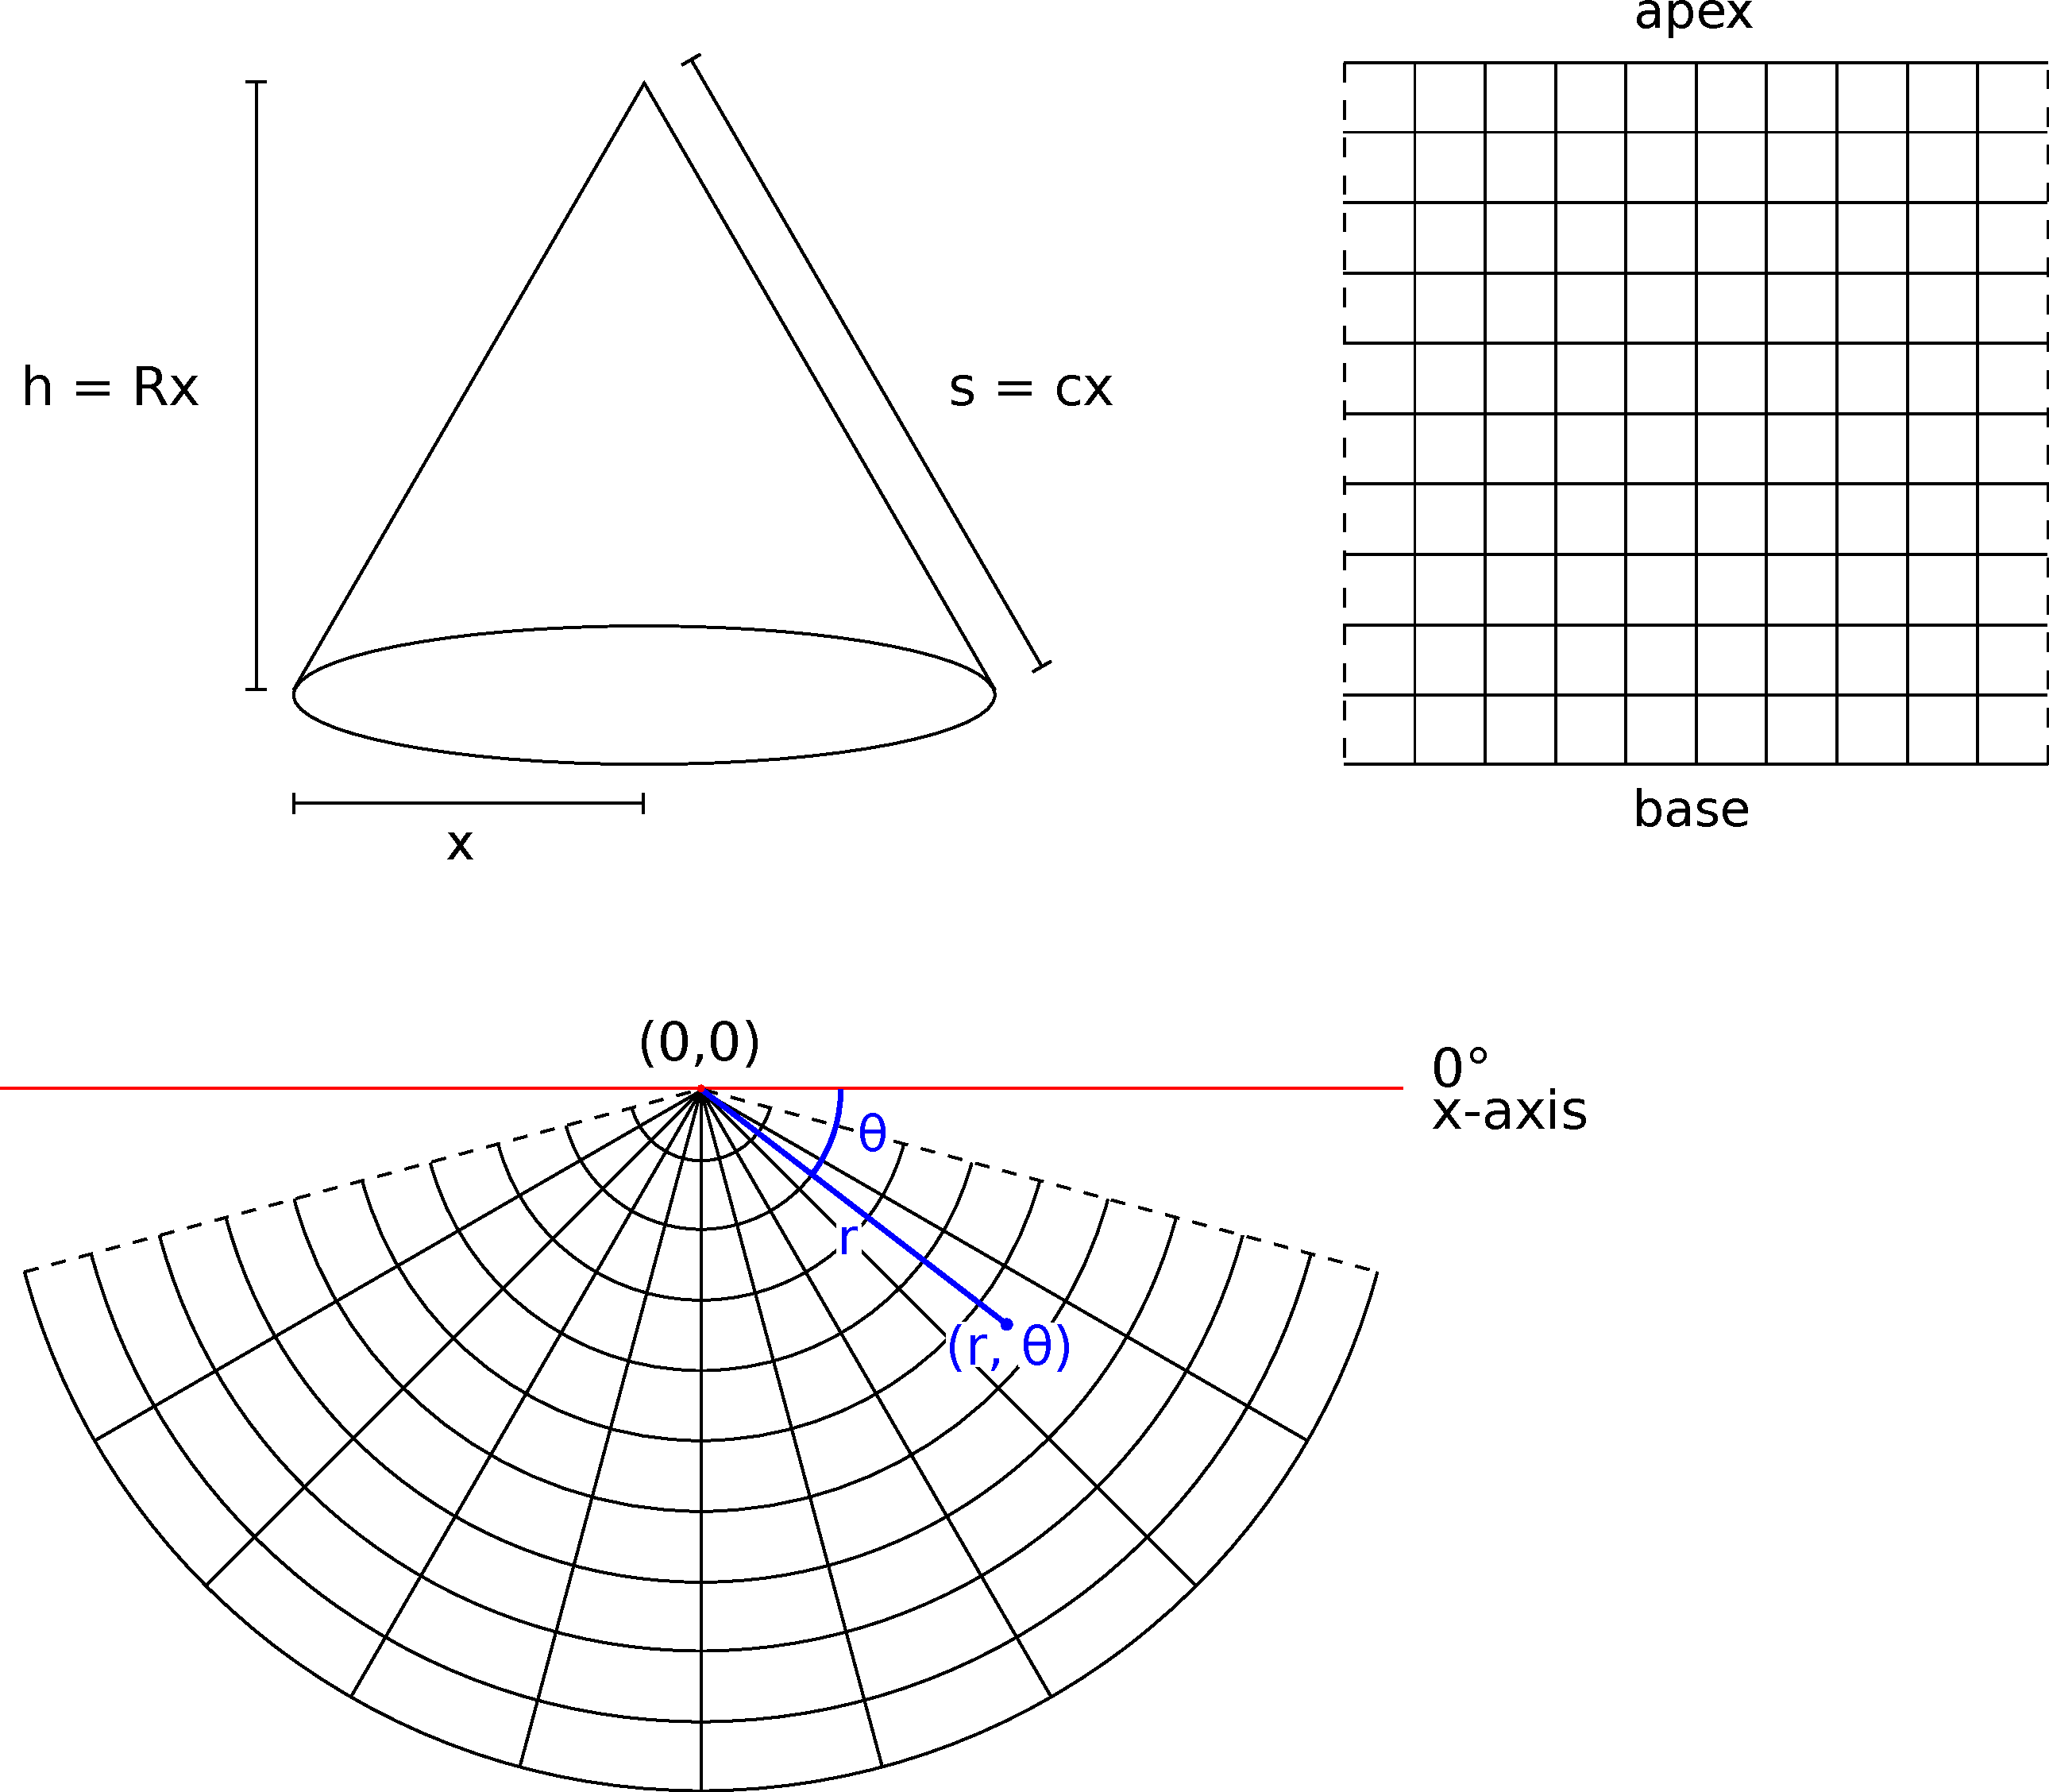
\includegraphics[width=1\linewidth]{ConeGrid_r_theta.pdf}

	\caption{\textbf{(A)} The model mountain is a cone, which has three parameters: base radius ($x$), height ($h$), and slant height ($s$). \textbf{(B)} Unfurled, a cone's surface is a circle sector. The polar coordinates, $r$ and $\theta$, describe position on the mountain. The circle centre (mountain tip or cone apex) is the origin, (0, 0). \textbf{(C)} In silico, I represent the cone's surface as a square array (grid of cells). Rows in the array are altitudinal bands, and columns, positions along a band. Row indices correspond to radial positions, and column indices, to angular positions. The array's top edge is the cone's apex (mountain tip).}
\label{Model}
\end{figure}

\subsection{Population Density}
Each cell in the array has $n$ individuals; $n$ is a function of body mass and area. Population density (number of individuals per unit area) should decline with body mass as $M^{-0.75}$, if resource supply is constant. This is because individual resource demand depends on metabolic rate, which increases with body mass as $M^{0.75}$. Observations in animals and plants support this \cite{enquist1998allometric, damuth1987interspecific}. A mountain base covers more area than the top. The model mountain is a cone, but, in silico, it is a square array. So, going up the mountain, each cell in the array represents an increasingly narrow area. If $A_c$ is cell area, the number of individuals in a cell is:

$$A_c M^{-0.75}$$

Then, the area of one cell in an altitudinal band is:  

$$\frac{\pi c \bigg(\Big(\frac{(I_r + 1)x}{T_r}\Big)^2 - \Big(\frac{I_r x}{T_r}\Big)^2 \bigg)}{T_\theta}$$

Cell area is unitless, and instead expressed in terms of x, keeping the model tractable. Please see the SI for the derivation of this equation.

\subsection*{Birth and Death Rates}
According to the Metabolic Theory of Ecology, metabolic rate (rate at which organisms process matter and energy) affects the rates of growth, reproduction, and dispersal, as well as the longevity of organisms \cite{2012Me:a} (Sibly et al 2012). Metabolic rate depends on the body size and temperature of organsisms - it increases as a power law with body size, and exponentially with temperature. Gillooly and Brown et al \cite{gillooly2001effects} combined previous work on the body-size and temperature dependence of metabolic rate into a single equation:
$$B = B_0 M^{\alpha} e^{\frac{-E}{kT}}$$

Temperature dependence is described by $E$, activation energy, k, the Boltzmann constant ($8.617 \times 10^{-5} eV K^{-1}$), and T, temperature in Kelvin. $M^{\alpha}$ is the power law describing the relationship between metabolic rate and body size. $B_0$ is a mass and temperature independent, normalisation constant, which accounts for other variation, and controls the vertical offset of the function. The value of the mass and temperature exponents can vary, but an interspecific average of $E$ is 0.65 \cite{allen2006kinetic, dell2011systematic} (Allen et al 2006, Dell et al 2011).

Each row of cells in my model has a temperature. The temperature sets the rate of birth, death, and dispersal. Accordingly, in my model, the probability of selecting an individual to die or reproduce is:

$$e^{\frac{-E}{kT}}$$

The per-cell probabilities are then normalised, so they sum to 1. I call the probabilities of birth and death across each position in the landscape the birth and death 'maps'.

\subsection*{Dispersal}
Individuals do not move, but species disperse via birth and death (when an individual reproduces, its offspring fills a gap vacant due to a death). An individual's chance of being chosen to reproduce depends on its birth rate, dispersal ability, and distance from the destination (vacant position). In other words, it is the net probability of birth and dispersal. The challenge is that, across space, birth and dispersal rates vary.

Imagine the origin of a dispersal kernel as being centered on the start point; the kernel describes the distribution of destinations. In a sense, in neutral models, the kernel is backwards, as it centered on the destination (position vacant due to death). From the kernel, the models pick a random distance and direction away from the vacant position. This picks the parent whose offspring occupies the vacancy. While convenient computationally, this only works if dispersal (and birth) rates are fixed. To vary dispersal rate, I must amend this usual algorithm. The solution is a set of 'dispersal maps'.

Before running a simulation, I calculate the probability of dispersing from every cell to the destination - a discrete probability distribution, which I call a dispersal map. As each cell is a potential destination and probability depends on distance, there is a map per cell.
Upon death, the model uses the maps to immediately pick a random parent. Dispersal maps are an elegant solution because they capture, in a single step of the model, variation in two traits, across three factors (temperature, body size, and area).

The model uses a standard normal distribution (mean = 0, standard deviation = 1) as a dispersal kernel. The distribution's scale parameter, $\sigma$, determines its spread - the likelihood of long-distance dispersal events. It has thin tails, meaning it predicts lower rates of long-distance dispersal than fat-tailed kernels (which curve away from the x-axis). Being a phenomenological kernel, it does not capture complex dispersal behaviour (Clobert et al 2012). But, it is a simple start point to introduce metabolically-driven (deterministic) variation to dispersal.

To apply a metabolic effect to dispersal, I multiply a distance, drawn from the kernel, by a body-size and temperature dependent parameter, $y$:

$$y = B_0 M^{0.25} e^{\frac{-0.65}{kT}}$$

$y$ is proportional to mean dispersal distance, and increases with body mass and temperature.

The array has two axes: one runs vertically across rows, the other horizontally across columns. Instead of drawing a random direction, a simple equivalent is to draw a distance along each axis separately. This is a unique, simplifying property of the normal distribution. It also allows me to study the contribution of dispersal vertically (up and down the mountain) and horizontally (round the mountain). Instead of drawing a random distance from the dispersal kernel, I use to it calculate the probability of dispersing a known distance, from a given destination.

\subsubsection*{Horizontal Dispersal}
Going up a mountain, the distance round it decreases (the base covers more area than the top). However, in silico, the system is a square array - horizontal dispersal distance must be adjusted. Towards the top, individuals should be more likely to disperse among cells, within a row (ignoring the effect of temperature). Also, they should be more likely to complete a revolution round the mountain. So, dispersal ability is unaffected by area, but, as area reduces going up, so does the distance among cells.

The model expresses distance in relative terms. This maximises the model's relevance (the simulated mountain can be any size) and minimises complexity (I need not pick absolute values for the cone's dimensions). An altitudinal band is a circle round the cone's surface. So, horizontal dispersal (left to right or vice versa) occurs along an arc of a circumference. The probability of dispersing the horizontal distance to the destination is:

$$P\Big(V = \frac{n_\theta x \pi (S_r + E_r)}{T_\theta T_r y}\Big)$$

Please see SI for derivation. This depends on distance to the destination (an arc, or proportion, of a circumference), body size, and temperature. It decreases as $V$ increases, as $V$ is a variate of the standard normal distribution (mean = 0). Probability increases as body size and temperature increase, and distance reduces. In other words, big individuals, and those in hot places or close to the destination, have a higher chance of reaching the destination.

\subsubsection*{Revolutions Round the Mountain}
So far, I assumed individuals take the shortest route between the start point and destination. This is not necessarily true because the array's left and right edges connect. So, to reach a given location, individuals can go in either direction (left or right). What is more, they can go via any - and a theoretically infinite - number of loops round the mountain.
I.e., they have a choice of alternative routes of varying distances. Accordingly, per horizontal position, I sum the probability of each alternative distance to the destination.

\subsubsection*{Vertical Dispersal}
Dispersal up and down the mountain occurs between the apex and base, along the cone's lateral (curved) surface.
Unlike the left and right edges, the bottom and top ones are not joined - individuals cannot disperse across them. So individuals can only disperse in one direction. The probability of dispersing up or down the mountain, from one row to another is:

$$P(V = \frac{n_r cx}{T_r y})$$

Like $d_\theta$, it depends on distance to the destination (a proportion of the slant height), body size, and temperature.

I multiply the probabilities of dispersing the horizontal and vertical distances, to get the probability of dispersing from every [row, column] position to the destination. For a given destination, I then multiply the dispersal rate (or probability) at each position with the position's birth rate. This produces a net probability of birth and dispersal, which I normalise so the probabilities sum to one. These map of net birth and dispersal rates are used to, upon a death, immediately pick an individual to reproduce - a spatial map of the possible parents for immigrants to that cell. Calculating these probabilities before running the simulation is a computationally tractable way to introduce variation in these key ecological rates.

\subsection*{Normalisation of Dispersal Rates}
$B_0$ is usually parameterised using taxon-specific regressions of trait on temperature. Here, however, I set it to be a free parameter. Increasing $B_0$ uniformly increases dispersal rates everywhere, and decreasing, vice versa. I set it to a moderate values that ensures dispersal is not dominated by:
1. looping round the mountain
2. dispersing within a single cell.

\subsection*{Thermal Optima and the Neutrality Assumption}
The rate of vertical dispersal is set by the temperature of the dispersal start point. (In later simulations, I instead change this to the temperature of the altitude halfway between the start and destination). However, as an individual disperses up or down the mountain, their temperature environment changes. Modelling a dynamically-changing effect of temperature on dispersal would involve combining successive transformations of the dispersal kernel. This is complex. 

The physiology of species limits the range of temperatures in which their survive. It is not necessarily realistic that, once a species disperses to a new temperature environment, their fitness is unchanged \cite{AngillettaMichaelJ.MichaelJames2009Ta:a}. To compensate for the mechanism of vertical dispersal, the model has a survival component. All individuals in the model have a temperature optimum ($T_{opt}$). An individual's $T_{opt}$ is:
- the temperature at which it is most likely to survive
- at the start of the simulation or for a new species, the temperature of its position
- otherwise, the same as its parent's.
The probability of surviving at different temperatures is a normal distribution; the mean of which is the $T_{opt}$ (highest probability of survival). Upon dispersal, the temperature of the destination is used to extract the probability of survival from the normal distribution. If an individual does not survive, the algorithm picks another individual to disperse, until the dispersing individual survives.

The scale parameter of the normal distribution is akin to thermal niche width, and defines a new parameter of the model. Increasing thermal niche width, would increase dispersal among altitudinal bands, and decreasing it, vice versa.

Individuals are no longer equivalent - the model is no longer neutral. As the thermal optimum is passed from parent to offspring, this property is not independent of species identity. It is important to note that species $T_{opt}$ do not change in the model, there is no adaptation or acclimation to new environments.

\subsection*{Parameter Space Analysis}
The model's parameters, in addition to the geometric ones in Table 1, are listed in Table 2. I begin with a basic neutral model with no temperature or area gradient. I then apply the following three effects independently and in concert with each other:
- metabolic effect on i) dispersal, and ii) birth/death, via a thermal gradient
- area gradient, which affects the distance round the mountain and the number of individuals per altitudinal band.
In this way, I could test the relative importance of dispersal and birth/death, and area and temperature.

I simulated the full model (with all effects) for body size values that span two orders of magnitude. Note that the absolute body-size values of these guilds is not important - it is the relative difference that is important. The reason is a computational limitation. There must be at least one individual per cell in the landscape - I normalise the scaling of abundance accordingly. Therefore, the model likely has unrealistic levels of abundances. So, the model is not designed to precisely predict the number of species, but can predict general trends and patterns.

Finally, I vary the following parameters:
- thermal niche width (standard deviation of a normal distribution)
- the ratio between the mountain's height and base radius, $R$, which controls the mountain's steepness
- the normalisation constant for dispersal, $B_0$
- speciation rate, $v$

Increasing the height or base radius of the mountain, leads to an increase in area and thus abundances of individuals. To keep the size of communities tractable, I fixed the area, but varied the mountain's steepness by varying the ratio of height to base radius. The default temperature gradient was 10-25 \degree C, which approximates that on a tropical mountain. I also uniformly decreased the mountain's temperature by 10 \degree C, to simulate a hypothetical temperate mountain. These parameters represent abiotic factors, and factors related to the species traits. Thus, I could also test whether any apparent general trends in diversity, changed under different scenarios.

I wrote code for the model and simulations in Python 3, and ran the simulations for 48 hours on the High Performance Computing Cluster at Imperial College London. I ran at least 10 replicates of each parameter combination. More replicates would be preferred - the number reflects what was possible in the project's time frame, given the number of parameter combinations.


\section*{Results}
\subsection*{Dispersal Maps: Hoes does the Pattern of Dispersal Change Going up the Mountain?}
In the absence of a temperature gradient, dispersal rate is the same everywhere. However, the area gradient (the mountain's conical geometry) affects distance round the mountain, and thus the probability of dispersing to a given cell. For a destination at the top, individuals from any side round the mountain are almost equally likely to disperse in (Figure \ref{DispMapAreaNoTemp}). The probability of dispersing to the destination is mostly unaffected by horizontal distance to the destination. This is because distance round the mountain is short. In contrast, the mountain base is wide - distances among cells are further. Immigration to a destination there, is only likely to occur from the same side of the mountain. While vertical distance to the destination is more important, the effect is mostly the same regardless of the destination altitude. A destination at the base receives slightly more immigrants that are vertically further away. This is because I normalise probabilities so they sum to one, and there is less horizontal dispersal.

Adding a temperature gradient increases the chance of receiving immigrants from altitudes lower than the destination (Figure \ref{DispMapTemp}). This is true regardless of destination altitude. Crucially, this contrasts with the effect of area alone. The cause is that temperature, and thus dispersal rates, reduce going up the mountain. Similarly to the area effect, a destination at the top is equally likely to receive immigrants from any side round the mountain (horizontal distance is unimportant). This is despite the colder temperature. However, for a destination at the base, horizontal dispersal increases. This suggests temperature drives the dispersal  pattern at the base, but area drives it at the top.

Bigger individuals disperse further. At all altitudes, in all directions, bigger organisms have a wider pool of immigrants (Figure \ref{DispMapBodySize}). Uniformly increasing the temperature of the whole mountain (studying the hypothetical tropical mountain, instead of the temperate one), has a similar effect (Figure \ref{DispMapTemp}). Visualising the dispersal maps helped to parameterise the model by identifying extreme scenarios. Increasing or decreasing by an order of magnitude the normalisation constant for dispersal (higher or lower dispersal rates overall), overrode the variation induced by area and temperature – but to different ends: By increasing it, the probability of dispersing to a destination is almost the same everywhere. Decreasing it largely restricted individuals to one cell (Figure \ref{DispMapB0}). %why
%% closing remark?

\newpage
\begin{figure}[!hbtp]
%\vspace*{-1cm}

	\begin{subfigure}{.5\textwidth}
		\centering
		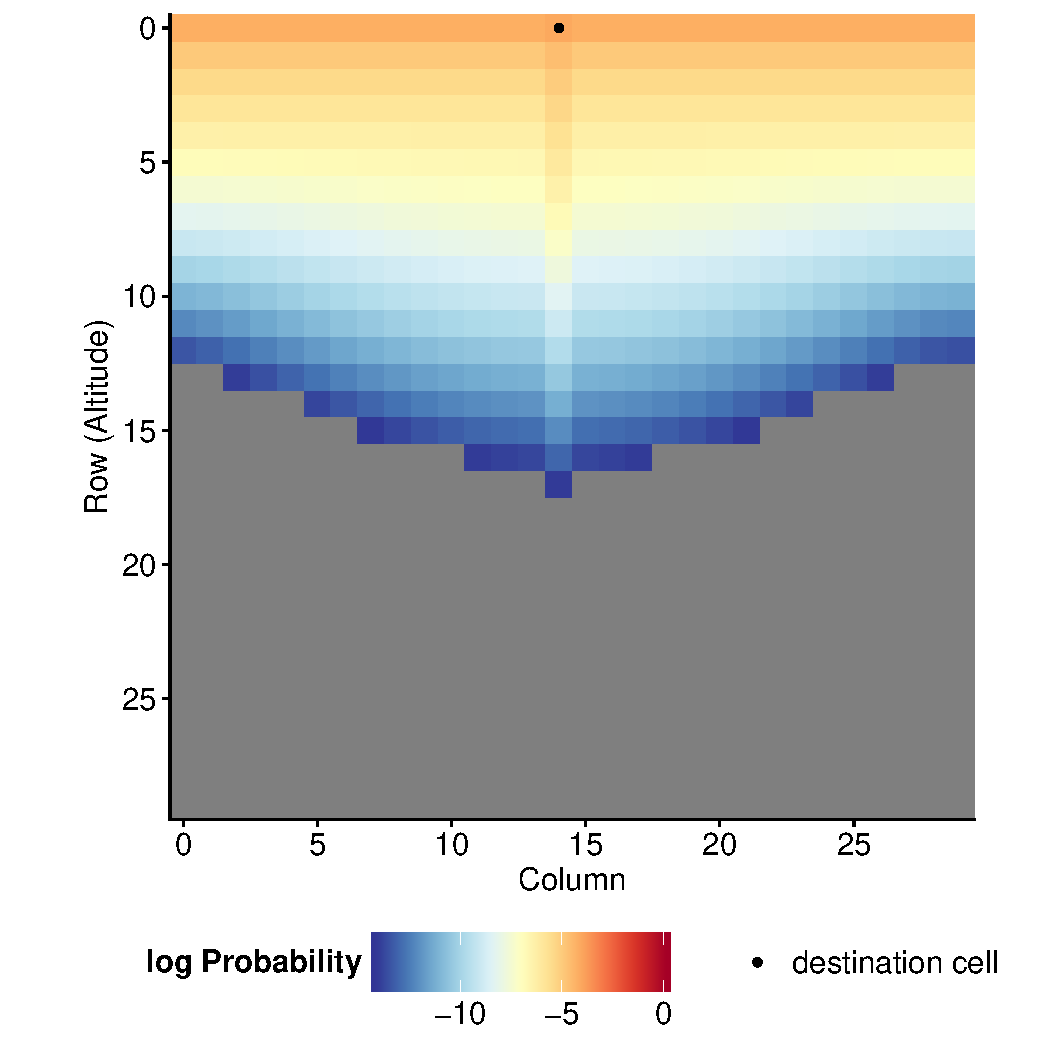
\includegraphics[width=1\linewidth]{../Results/DispMaps/AreaNoTemp100Top.pdf}
	\end{subfigure}
	\begin{subfigure}{.5\textwidth}
		\centering
		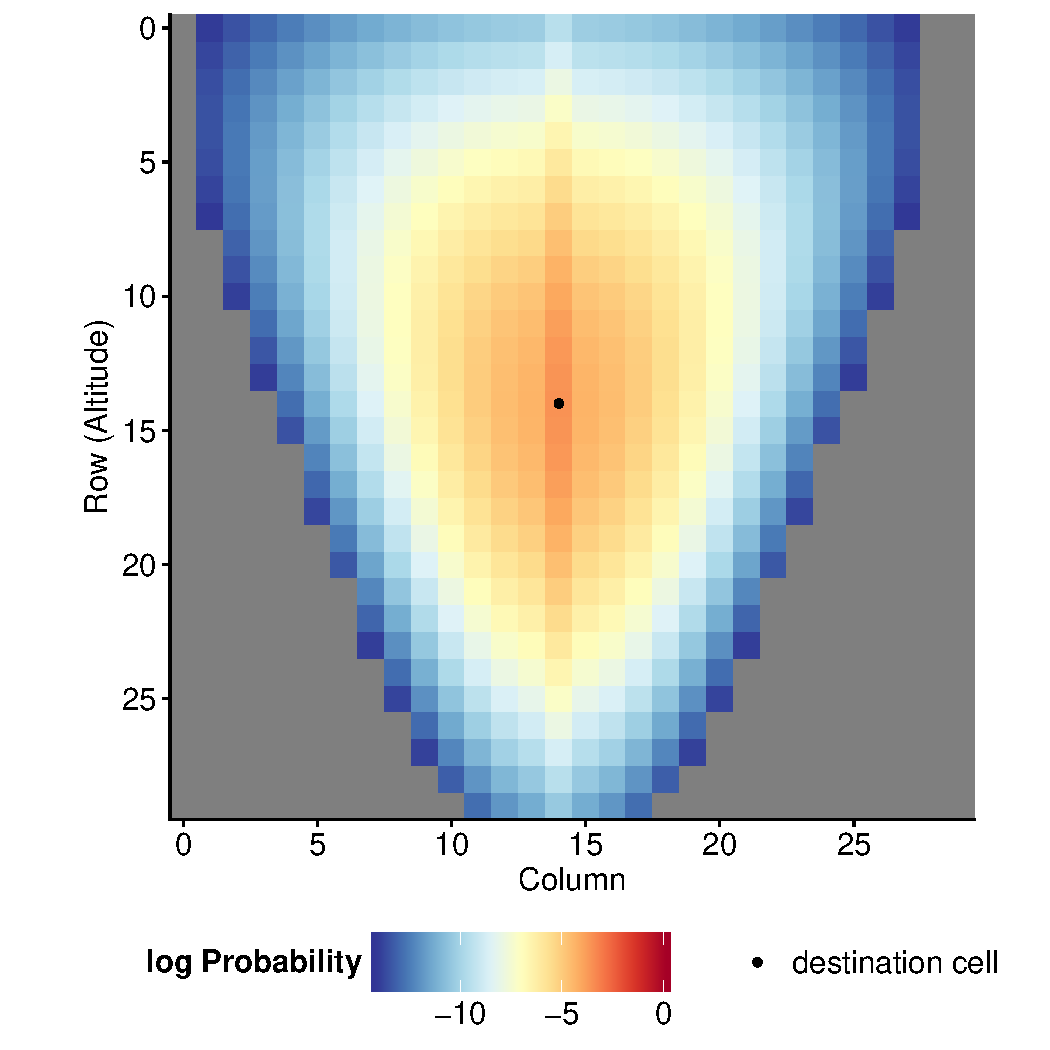
\includegraphics[width=1\linewidth]{../Results/DispMaps/AreaNoTemp100.pdf}
	\end{subfigure}
	
	\begin{subfigure}{\textwidth}
		\centering
		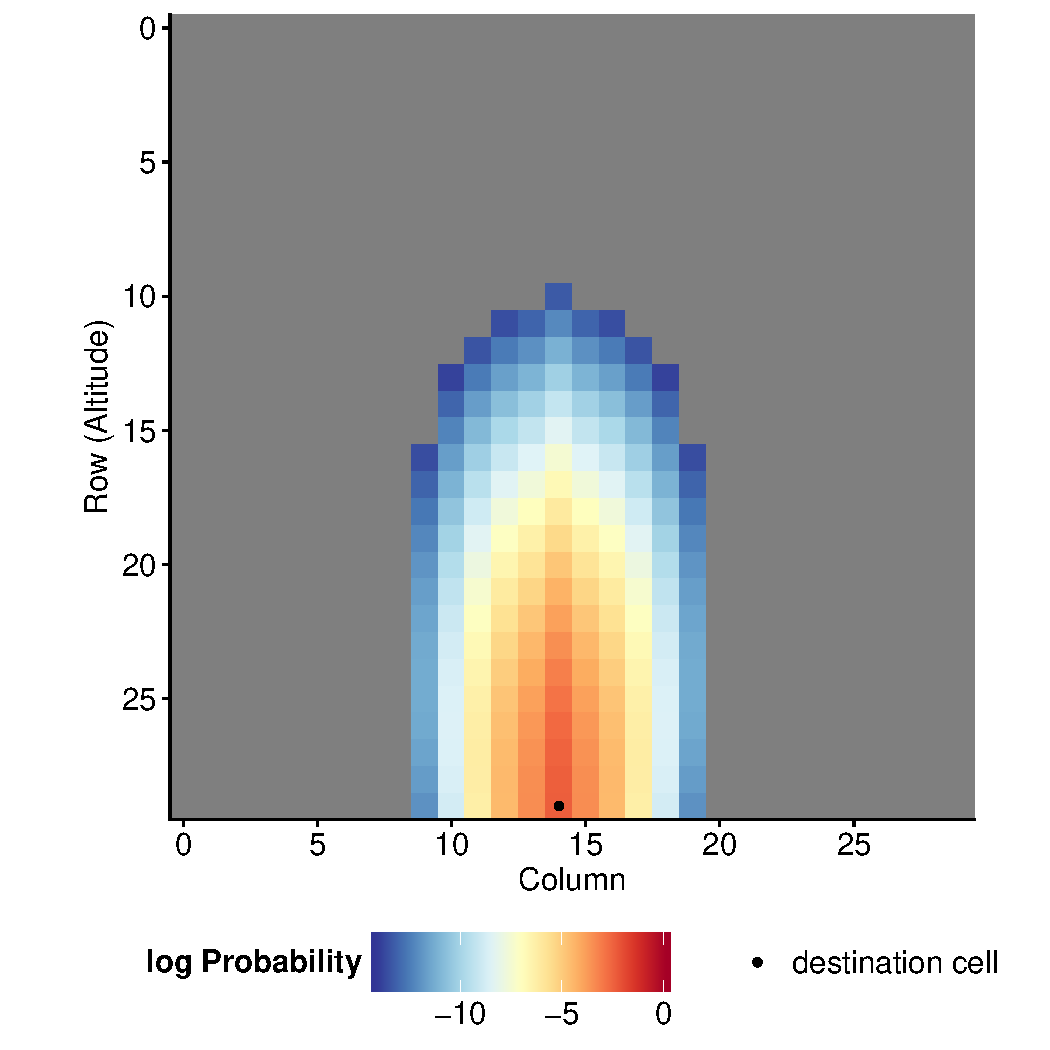
\includegraphics[width=0.5\linewidth]{../Results/DispMaps/AreaNoTemp100Bottom.pdf}
	\end{subfigure}

	\caption{\textbf{Dispersal Patterns on a Model Mountain - the Effect of Area.} Temperature is the same everywhere (15 \degree C). The heat map shows the probability of dispersing to a destination at the top, middle, and bottom of the mountain. Grey cells represent probabilities $\leq 1 \times 10^{-6}$. A mountain base covers more area than the top. But, in silico, the model mountain is a square array; going up it, each cell represents an increasingly narrow area. Row 0 is the top. Other parameter values: body size, $M$ = 100 g; ratio of the mountain's height and base radius, $R$ = 1.5.}
\label{DispMapAreaNoTemp}
\end{figure}


\newpage
\begin{figure}[!hbtp]

	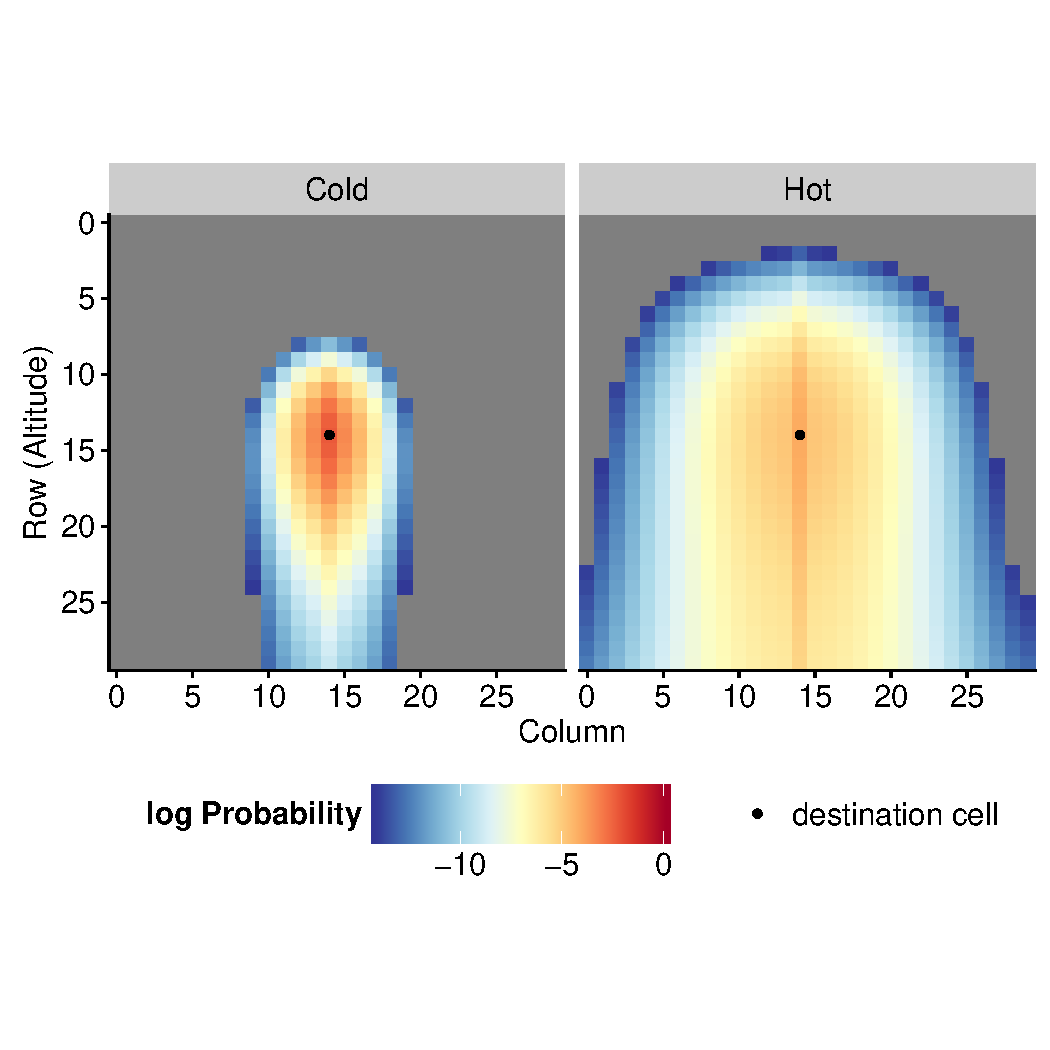
\includegraphics[width=1\linewidth]{../Results/DispMaps/AreaTemp_ColdHot.pdf}
	\vspace*{-3cm}
	\caption{\textbf{Dispersal Patterns on Model Mountains - the Effect of Temperature.} In the left plot, the temperature gradient approximates that on a temperate mountain (0-15 \degree C from top to base); on the right, a tropical mountain (10-25 \degree C). Temperature affects dispersal rate as per the Metabolic Theory of Ecology. The heat maps show the probability of dispersing to a mid-altitude destination. Grey cells represent probabilities $\leq 1 \times 10^{-6}$. A mountain base covers more area than the top. But, in silico, the model mountain is a square array; going up it, each cell represents an increasingly narrow area. Row 0 is the top. Other parameter values: body size, $M$ = 100 g; ratio of the mountain's height and base radius, $R$ = 1.5.}
\label{DispMapTemp}
\end{figure}


\newpage
\begin{figure}[!hbtp]
		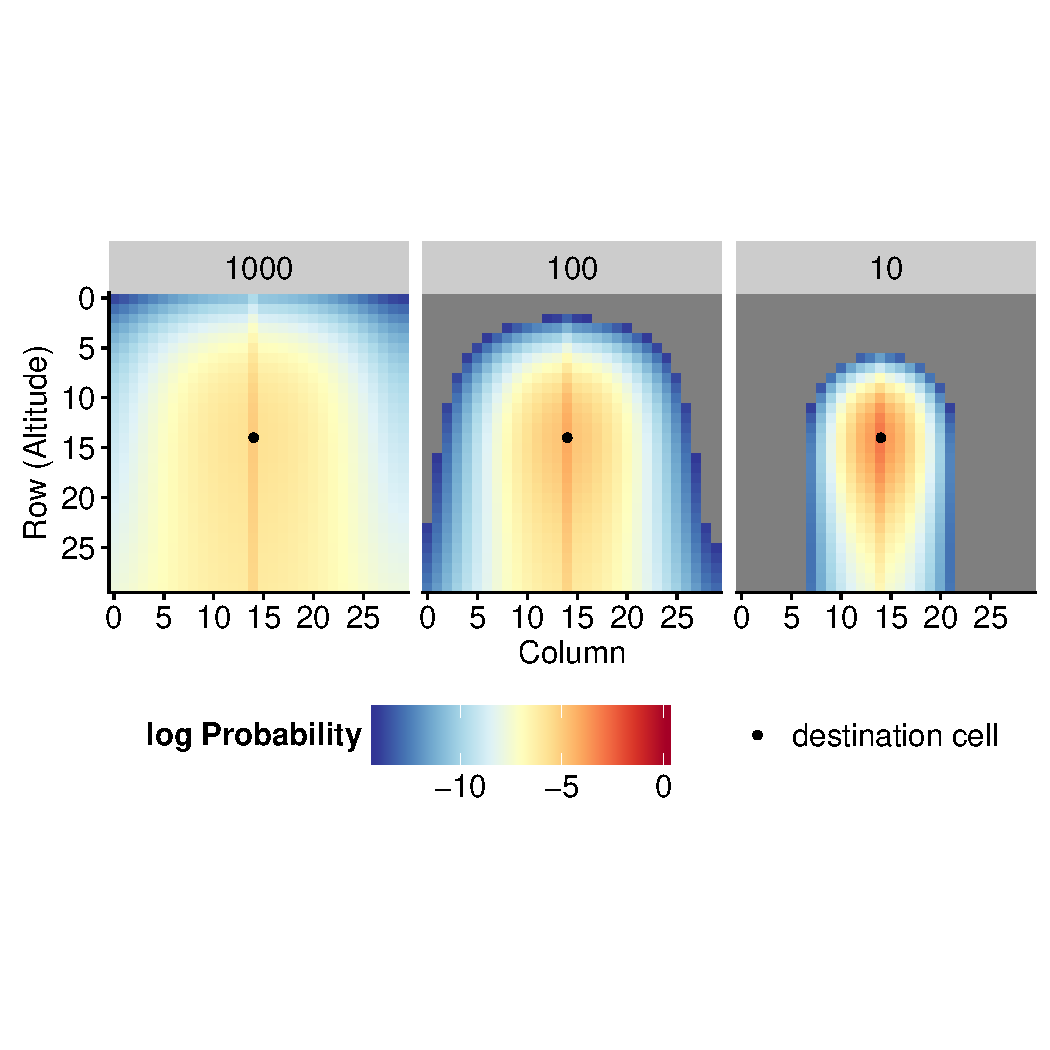
\includegraphics[]{../Results/DispMaps/AreaTemp.pdf}
		\vspace*{-4cm}
		\caption{\textbf{Dispersal Patterns on a Model Mountain - the Effect of Body Size.} Body size and temperature affect dispersal rate as per the Metabolic Theory of Ecology. The heat maps show the probability of dispersing to a mid-altitude destination. Grey cells represent probabilities $\leq 1 \times 10^{-6}$. The body sizes are 1000, 100, and 10 g, from left to right. The temperature gradient approximates that on a tropical mountain (10-25 \degree C). A mountain base covers more area than the top. But, in silico, the model mountain is a square array; going up it, each cell represents an increasingly narrow area. Row 0 is the top. Other parameter values: body size, $M$ = 100 g; ratio of the mountain's height and base radius, $R$ = 1.5.}
\label{DispMapBodySize}
\end{figure}


\newpage
\begin{figure}[!hbtp]

	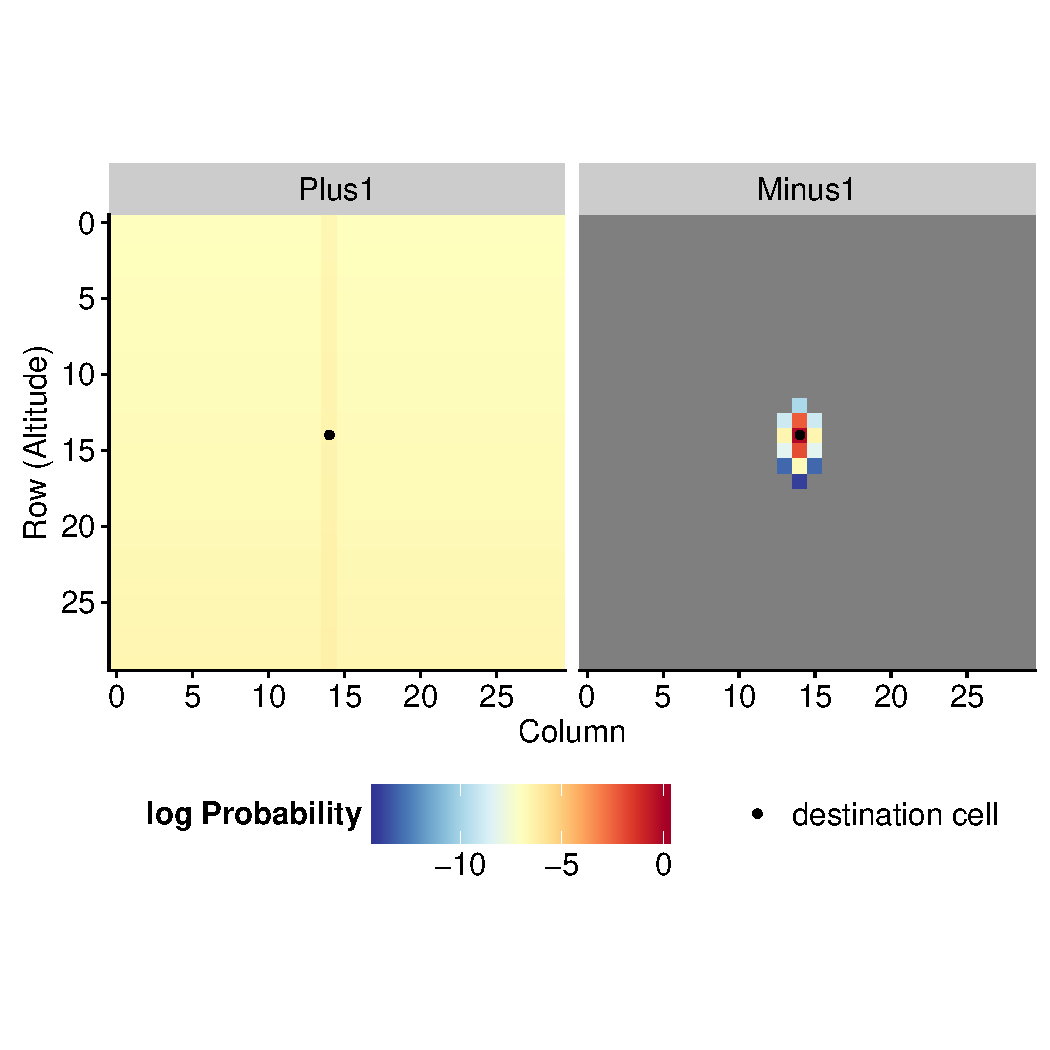
\includegraphics[width=1\linewidth]{../Results/DispMaps/AreaTemp_B0.pdf}
	\vspace*{-3cm}
	\caption{\textbf{'Making Mountains Out of Molehills': Dispersal Patterns on a Model Mountain, under Extreme Parameters.} Temperature affects dispersal rate as per the Metabolic Theory of Ecology. For the left plot, I increased the normalisation constant for dispersal by an order of magnitude. For the right, I reduced it by an order. The heat maps show the probability of dispersing to a mid-altitude destination. Grey cells represent probabilities $\leq 1 \times 10^{-6}$. The temperature gradient approximates that on a tropical mountain (10-25 \degree C). A mountain base covers more area than the top. But, \emph{in silico}, the model mountain is a square array; going up it, each cell represents an increasingly narrow area. Row 0 is the top. Other parameter values: body size, $M$ = 100 g; ratio of the mountain's height and base radius, $R$ = 1.5.}
\label{DispMapB0}
\end{figure}


\newpage
\subsection*{Altitudinal Biodiversity Gradients}
A basic neutral model, which had no temperature and area mechanisms, did not produce a biodiversity gradient at dynamic, extinction-speciation equilibrium. Rows in the array had a similar species richness, but with some stochasticity. Running the model, but with a metabolic effect on birth and death rate, via a thermal gradient, produced similar results.

By adding a metabolic effect on dispersal rate, an equilibrium gradient emerged - the species richness curve was hump-shaped (Fig. \ref{AltGradTemp}). Diversity was highest and plateaued along a wide, mid-elevational portion (the curve did not have a pointed peak), and declined towards the base and top. The gradient was consistent for diversity metrics, but, for gamma diversity, the gradient was stronger than for alpha. Mean gamma values at mid-elevation were twice those at the base; for alpha, the difference was 1.5 times. The trend in beta diversity was extremely weak, though consistent - a difference in the probabilities of only 0.06. Diversity at the base and top were similar, but, except for beta, the top was slightly and consistently more specious.

When I applied an area gradient (with no temperature variation), the diversity metrics showed different trends (Fig. \ref{AltGradArea}). For alpha diversity, the species richness curve was almost horizontal, before reducing about a fifth of the way up the mountain. Mean values at the base were twice those at the top. Gamma diversity, however, declined consistently, in a non-linear, monotonic way. Mean values at the base were 18.2 times those at the top - again, a stronger gradient than alpha. In stark contrast, beta diversity, and gamma per unit area, increased with altitude.
%
(Beta diversity is the probability that individuals, within a band, on opposite sides of the mountain, are the same species. A low probability means high diversity.) Unlike the temperature model, the beta-diversity gradient was strong. At the mountain top, cells within an altitudinal band had almost completely different species to each other (probability close to 0). Per unit area, gamma diversity at the top was 3.2 times that of the base. So, in terms of number of species, local and regional diversity declined. But, the opposite was true, per unit area, and when looking at how well-mixed species within a band were.

When modeling the temperature and area gradients together, their effects seemed to combine (Fig. \ref{AltGrad}). On alpha and gamma diversity, the effect seemed additive: diversity reduced with altitude, but peaked at a low-to-mid elevation, not the base. Whereas gamma declined linearly from the peak richness, alpha declined non-linearly, decreasing faster towards the top. Per unit area, gamma diversity resembles the hump-shaped gradient of the temperature model. The addition of an increase at the top reflects that seen in the area model. Beta diversity (especially at the base and through mid-elevations) is similar to the temperature model. The dissimilarity to the gradient in the area model, suggests an interaction between area and temperature for beta diversity. What is more, in the area model, beta diversity at the mountain top was very high. While in the temperature model it was low, here it is even lower. The potential interaction effect is in contrast to the other metrics, but must be verified by further investigation.

The patterns of alpha, beta, and gamma diversity were very consistent across body size guilds (I only varied body size in the combined model), though the exact number of species increased with decreasing body size - i.e., curves were shifted vertically. The hypothetical temperate mountain (uniformly decreasing the temperature by 10 \degree C) also showed no deviation, neither did increasing nor decreasing the mountain’s steepness. Increasing the normalisation constant for dispersal (higher dispersal rates overall - probability of dispersing to a destination is almost the same everywhere), only produced a slight increase, at the top, in beta diversity and gamma per unit area.

Some parameter combinations did alter the patterns. Most notably, increasing thermal niche width by an order of magnitude to 10, produced the same patterns as those in the area model. However, decreasing thermal niche width by an order of magnitude to 0.1, accentuated the patterns of the combined model. For alpha and gamma diversity, the low-to-mid elevation peak disappeared, and the trends were more linear. While the total number of species decreased, the proportional difference between the top and base increased. Mean gamma values at the base were 41 times those at the top; for alpha, it was 11 times. But for a sharp increase at the top, beta diversity, and gamma per unit area mostly did not differ across altitudinal bands. So the mid-elevation plateau for gamma per unit area disappeared.

In contrast to increasing it, decreasing the normalisation constant for dispersal () pronounced the strength of the gradients in alpha and beta diversity (but had no effect on gamma) - the decline towards the top was more marked. Beta diversity at the base strongly increased (the probability changed from 0.21 to 0.02 - higher values mean lower diversity). It remained low at the top and reduced slightly (0.36 instead of 0.33). The result of decreasing diversity towards the top on gamma per unit area was a slight peak at mid-to-low elevations, instead of a horizontal plateau. The increase at the very top (after the plateau’s decline) was still present, though the increase was no longer to a maximum.

In summary, when applied independently, area and temperature have different effects. The temperature model produced a plateau in richness at mid-elevations, across metrics. In contrast, the area model showed a decrease with altitude in alpha and gamma - but an increase in beta diversity. Applied in concert, the effects were additive, but beta diversity resembled that in the temperature model. For beta, this suggests an interaction between area and temperature. The trends of the combined model were consistent across many parameter combinations. Notable exceptions were increasing the thermal tolerance of species, and decreasing the normalisation constant for dispersal. This implies, under these conditions, the balance between the area and temperature effects changed.


\begin{figure}[!hbtp]
\vspace*{-3cm}
\centering
	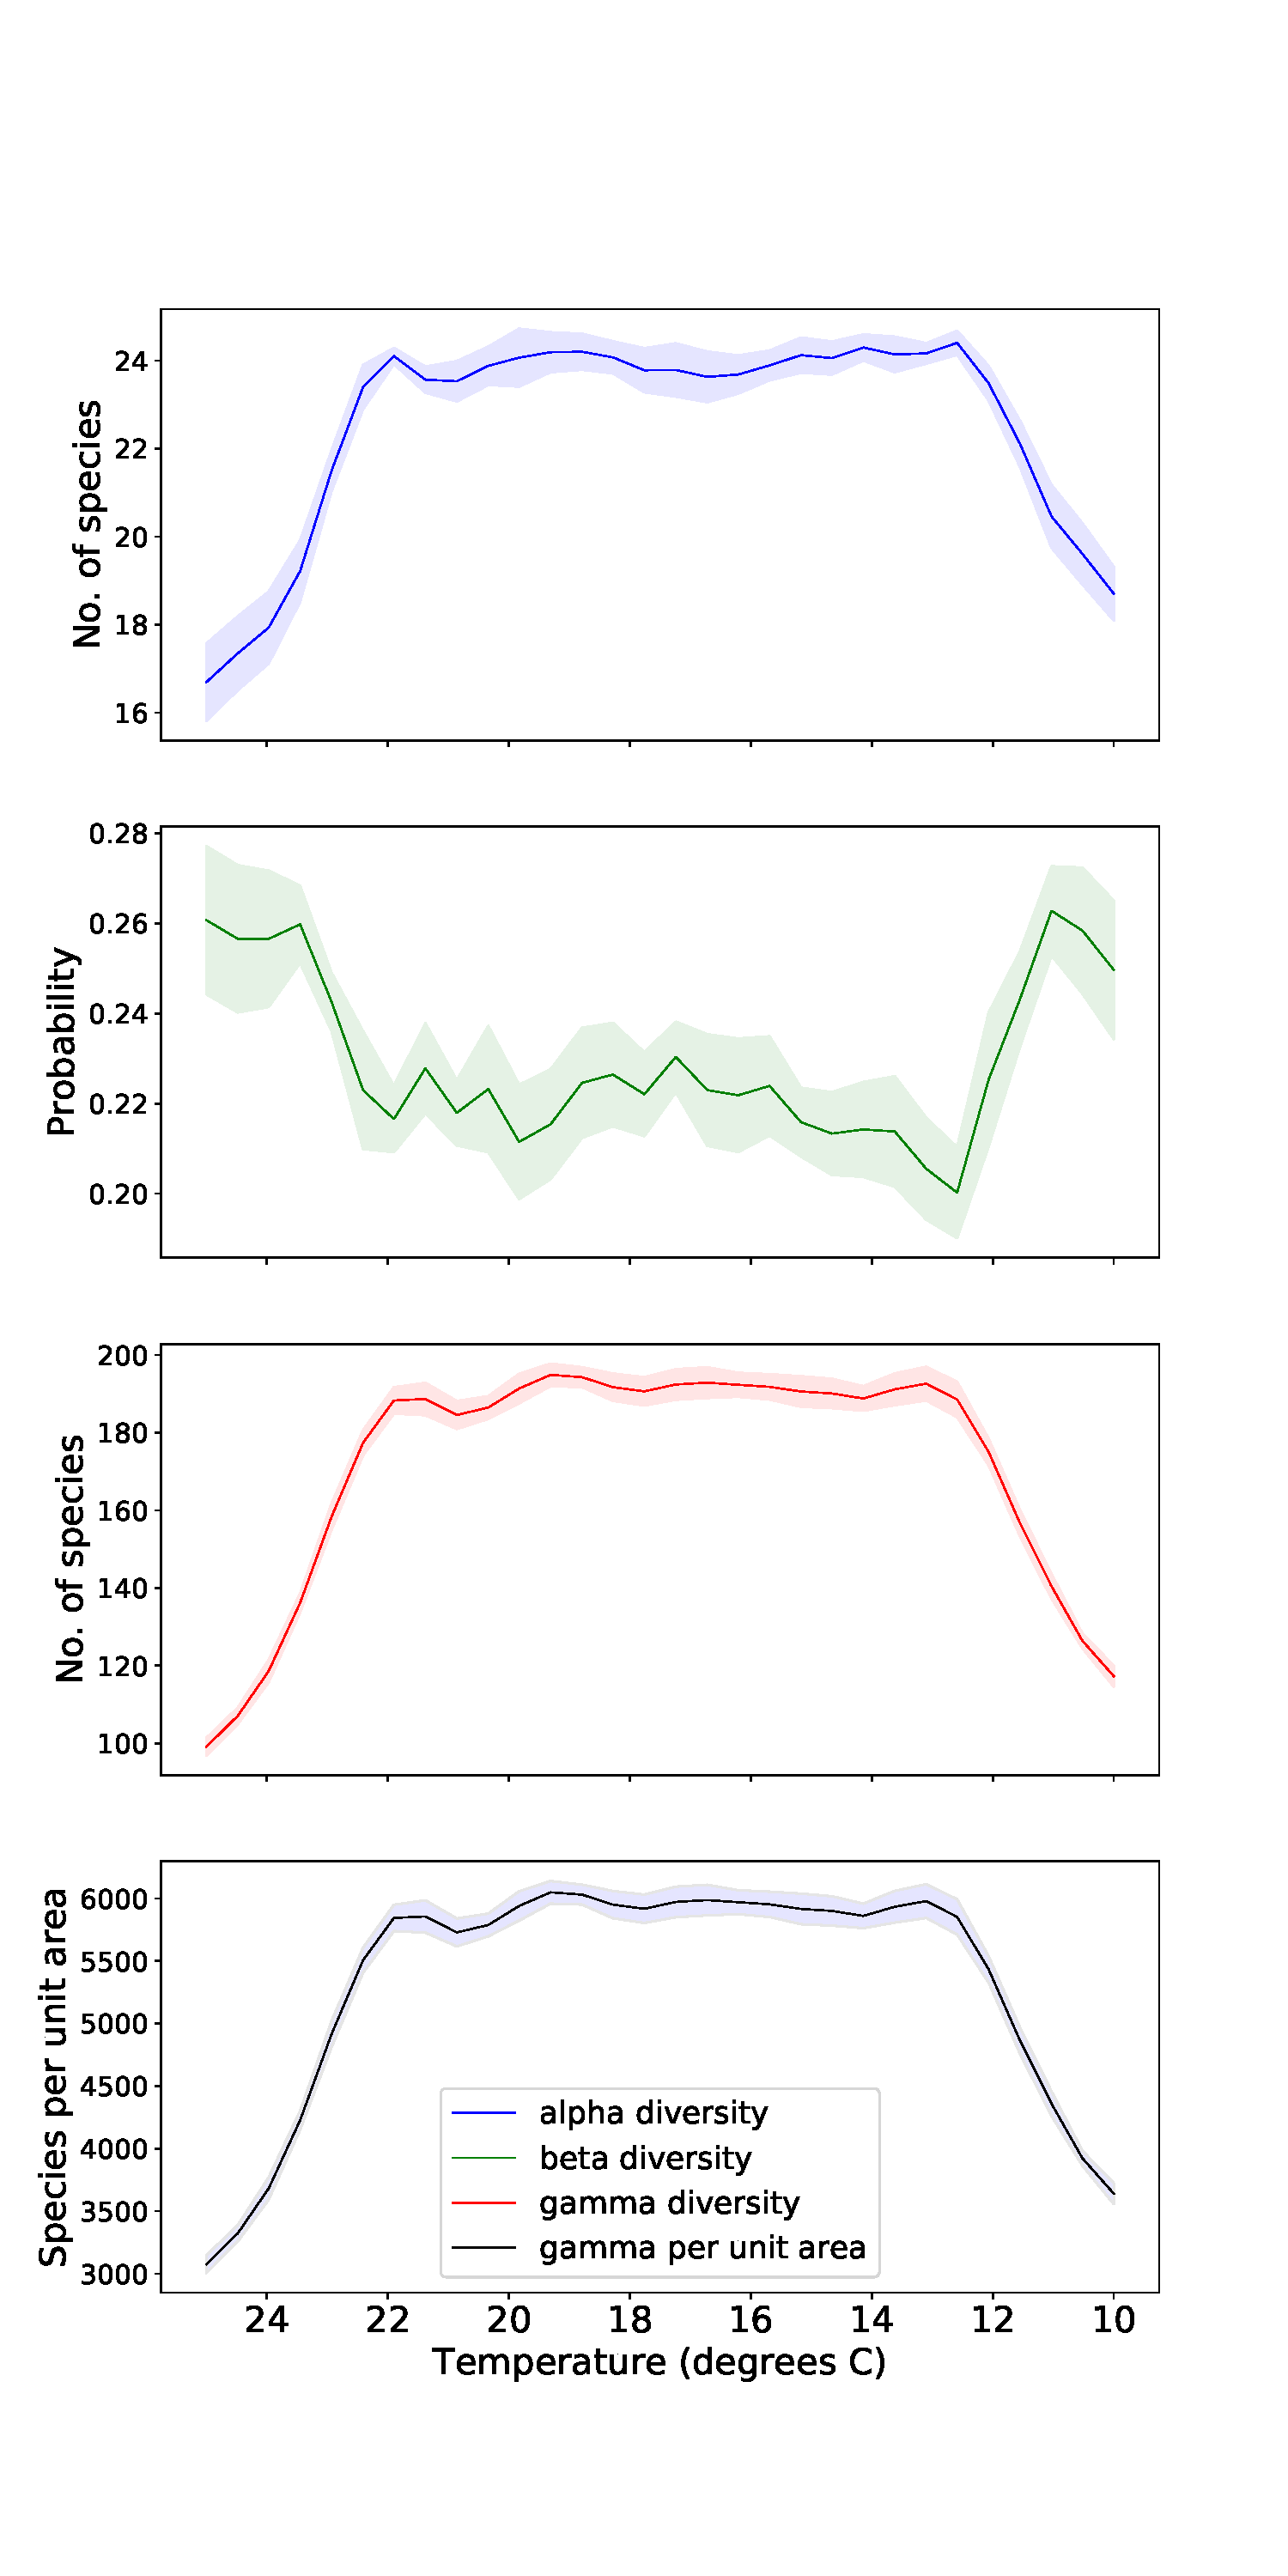
\includegraphics[width=0.6\linewidth]{../Results/DiversityPlots/TempNoArea.pdf}
	\vspace*{-1.5cm}
	\caption{\textbf{The Effect of a Temperature Gradient on Biodiversity.} The gradient approximates that on a tropical mountain (10-25 \degree C from base to top). Area, however, is fixed along the gradient (the model system is actually a cylinder, not a cone). Temperature affects birth, death, and dispersal rates as per the Metabolic Theory of Ecology.\\
	\\Each row of cells in the system has a temperature. The plot shows alpha, beta, and gamma diversity per row, and gamma diversity divided by row area - a proportion of the cylinder’s surface area. Solid lines indicate means, and shading, 95\% confidence intervals. Alpha (local) diversity is the mean number of species per cell. Beta diversity, the probability that individuals on opposite sides of the cylinder are the same species (high probability means low diversity). Gamma diversity, the total number of species.\\
	\\Other parameter values are the defaults: body size, $M$ = 1000 g; community size, 27 000 individuals; speciation rate, $v$ = 0.01; ratio of the mountain's height and base radius, $R$ = 1.5.}
\label{AltGradTemp}
\end{figure}


\begin{figure}[!hbtp]
\vspace*{-3cm}
\centering
	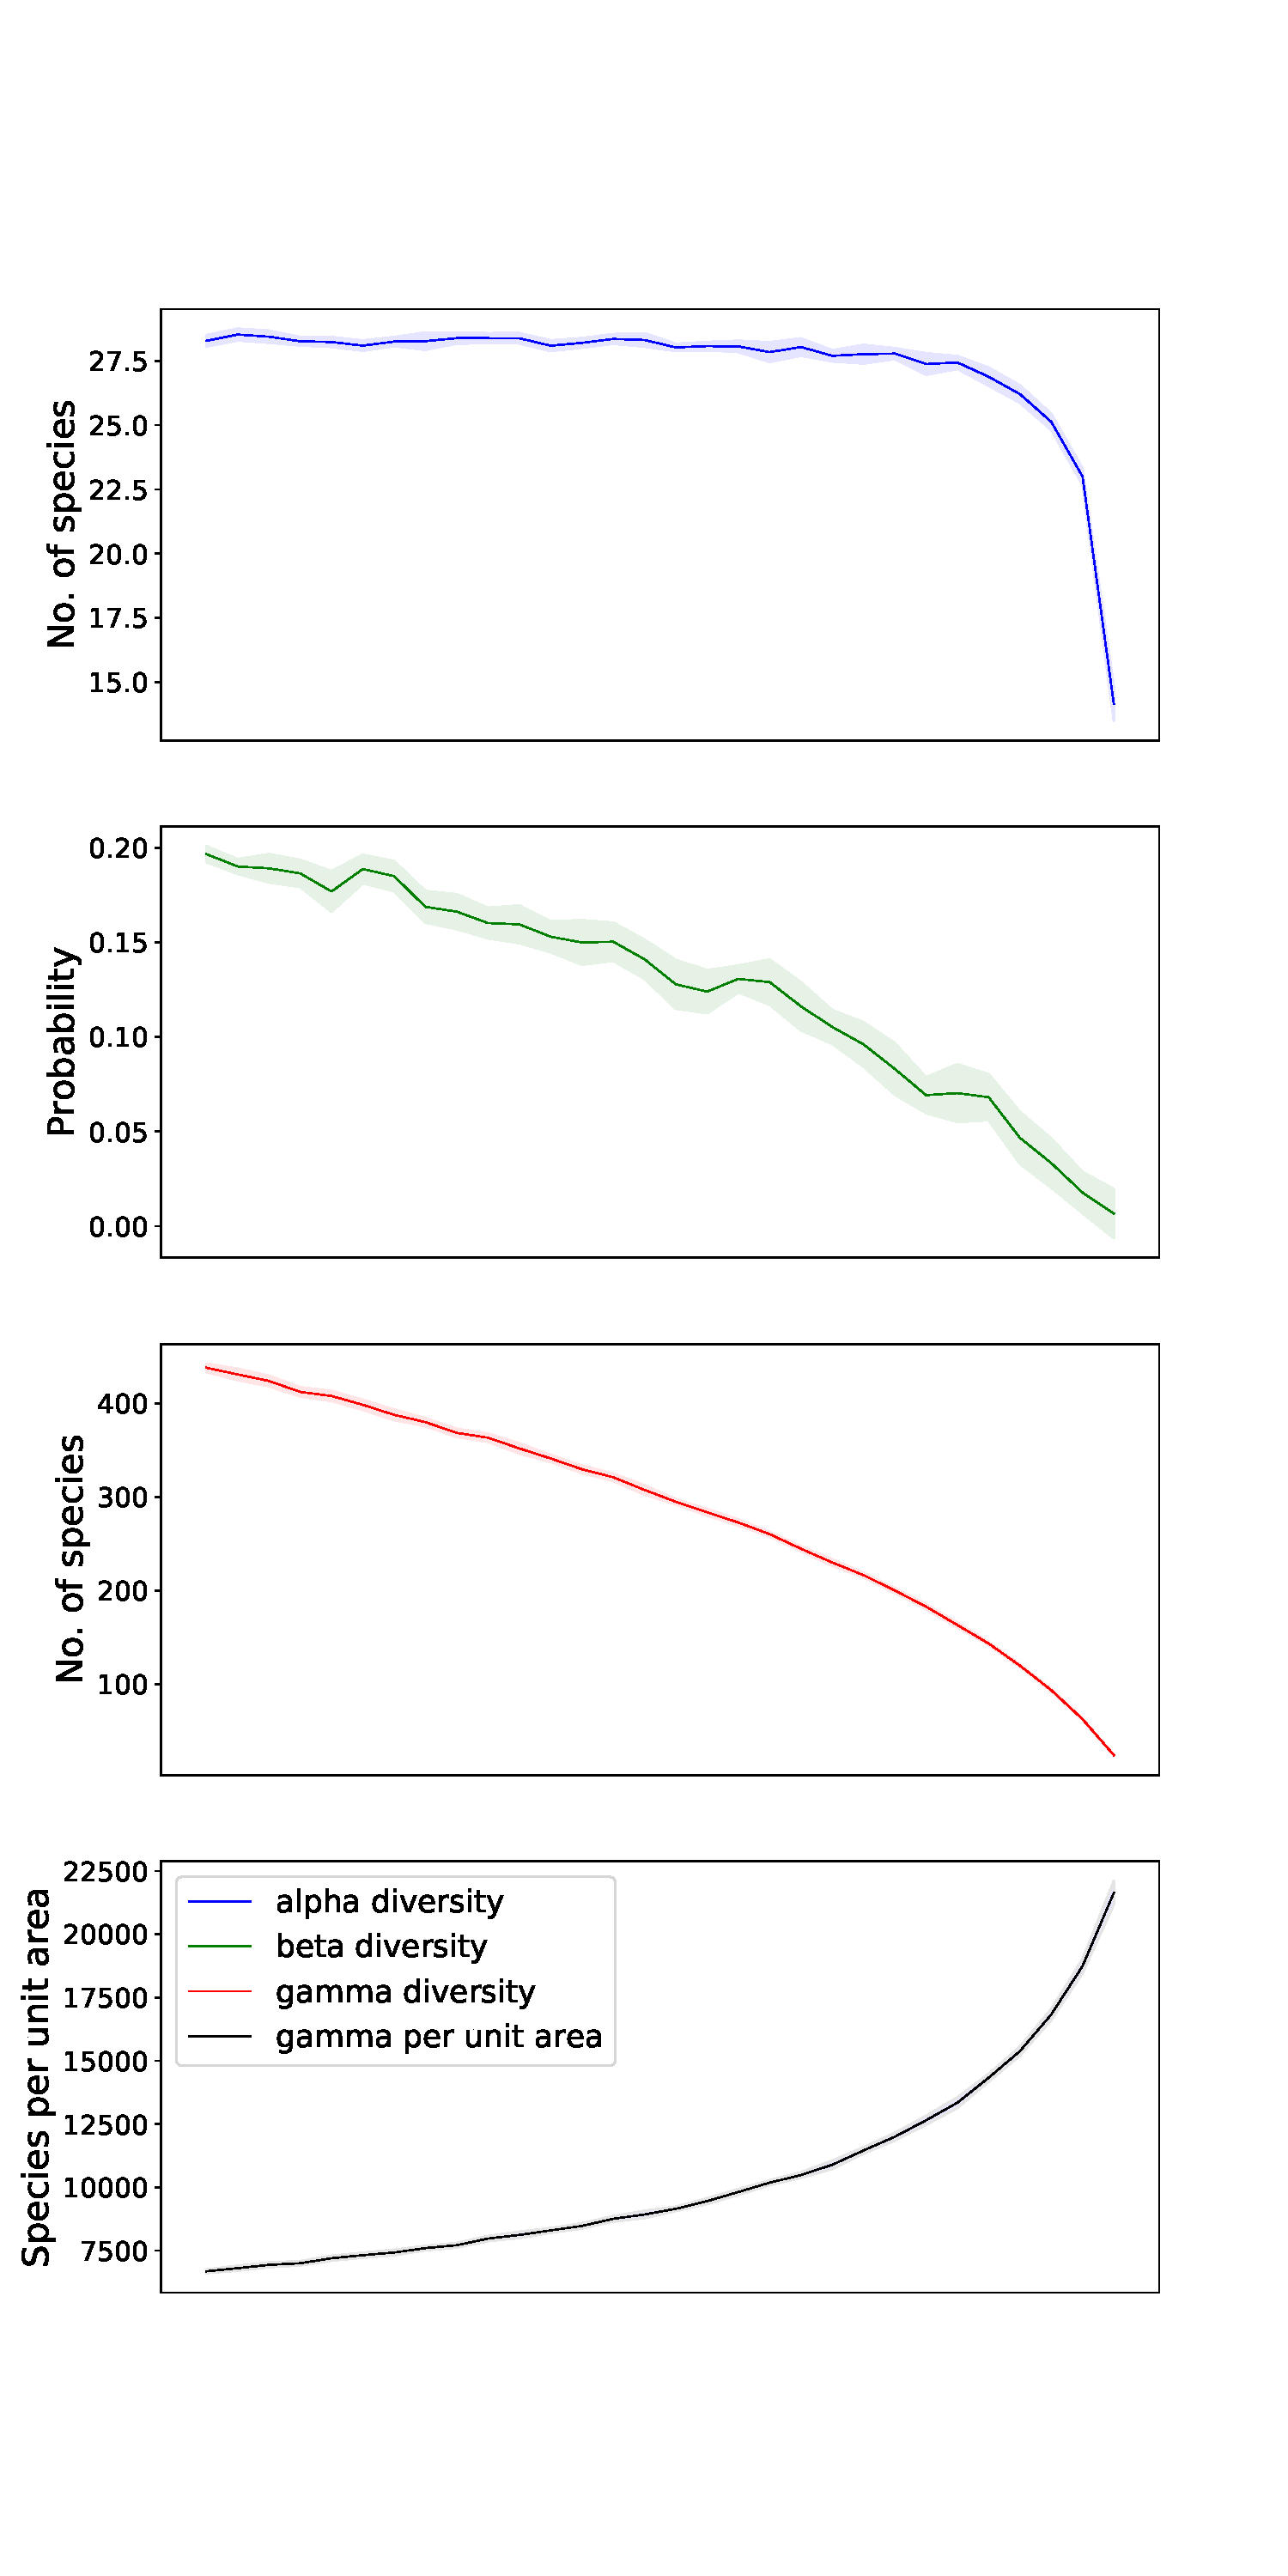
\includegraphics[width=0.6\linewidth]{../Results/DiversityPlots/AreaNoTemp.pdf}
	\vspace*{-2cm}
	\caption{\textbf{The Effect of Area on Altitudinal Biodiversity Gradients.} Temperature is the same everywhere (15 \degree C). The model mountain is a cone - the base covers more area than the top. But, in silico, it is a square array; going up the mountain, each cell in the array represents an increasingly narrow area. Area has two effects, going up the mountain: 1) There are fewer individuals per altitudinal zone (population density is fixed, but area reduces). 2) The dispersal distance among cells reduces.\\
	\\The plot shows alpha, beta, and gamma diversity per altitudinal band, and gamma diversity divided by band area - a proportion of the cone's surface area. Solid lines indicate means, and shading, 95\% confidence intervals. Alpha (local) diversity is the mean number of species per cell. Beta diversity, the probability that individuals on opposite sides of the mountain are the same species (high probability means low diversity). Gamma diversity, the total number of species.\\
	\\Other parameter values: body size, $M$ = 1000 g; community size,+ 27 000 individuals; speciation rate $v$ = 0.01; ratio of the mountain's height and base radius, $R$ = 1.5.}
\label{AltGradArea}
\end{figure}
% The effect of area without temperature. (Temperature fixed to 15 \degree C; body mass 100 g.)


\begin{figure}[!hbtp]
\vspace*{-3cm}
\centering
	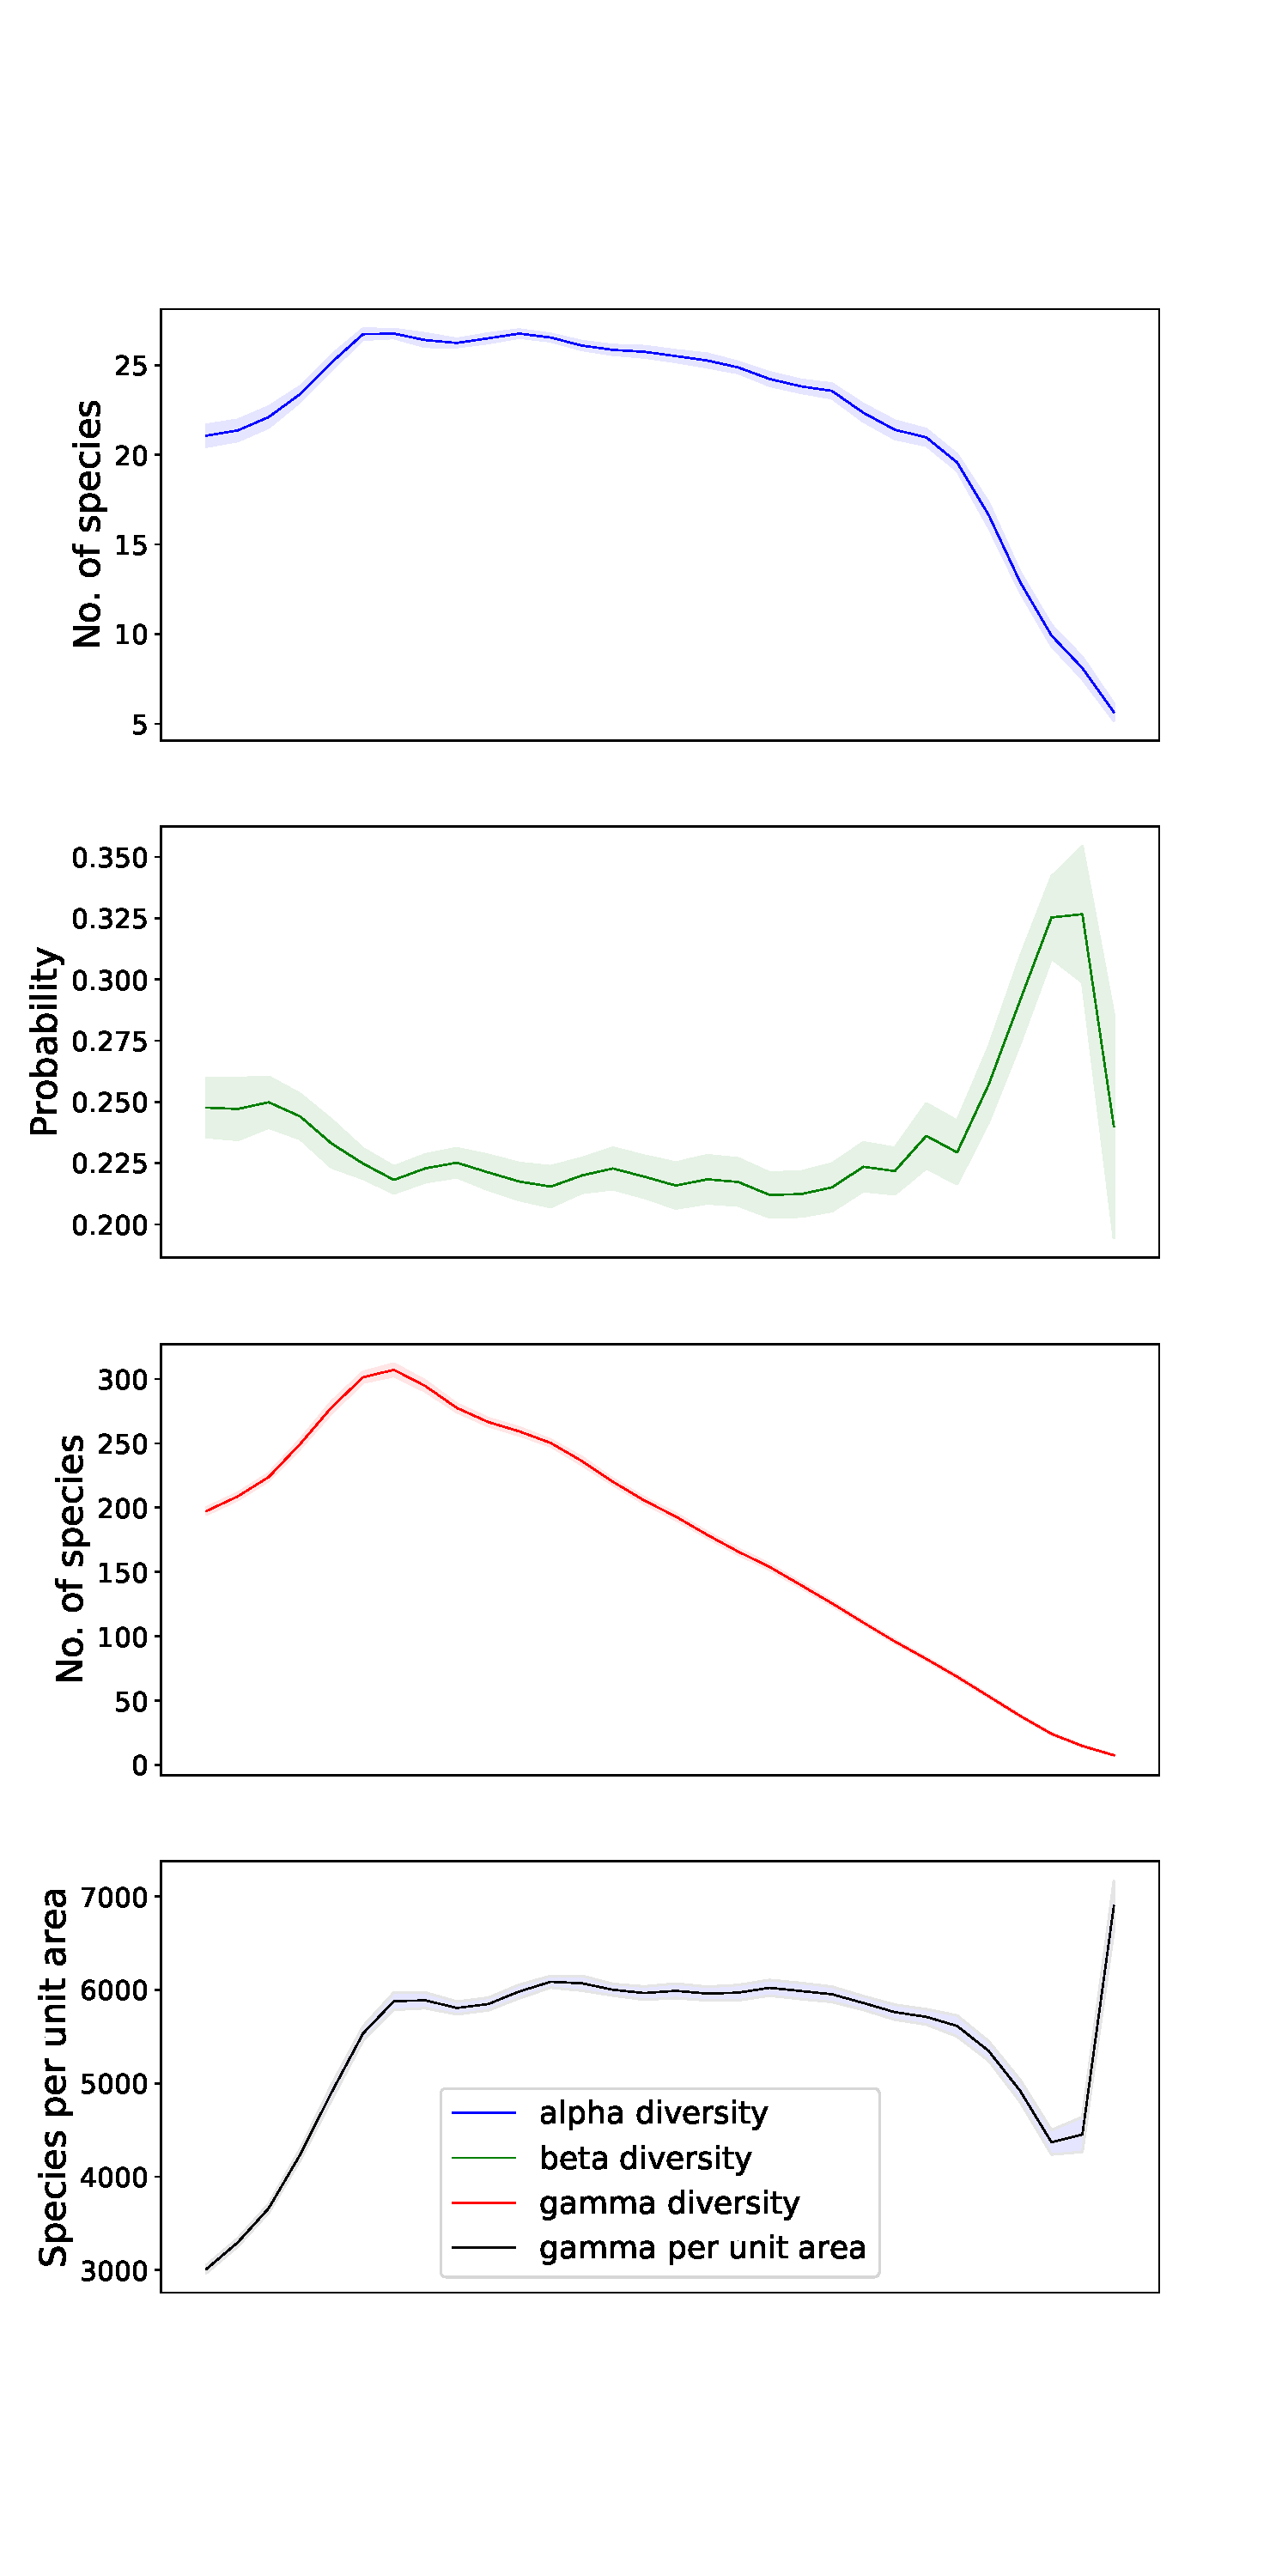
\includegraphics[width=0.6\linewidth]{../Results/DiversityPlots/1000.pdf} % 100
	\vspace*{-1.5cm}
	\caption{\textbf{Altitudinal Biodiversity Gradients.} Area reduces going up the mountain. Thus, the number of individuals, and dispersal distance among cells, reduce. The temperature gradient approximates that on a tropical mountain: 10-25 \degree C from base to top. Temperature affects birth, death, and dispersal rates as per the Metabolic Theory of Ecology.\\
	\\The plot shows alpha, beta, and gamma diversity per altitudinal band, and gamma diversity divided by band area - a proportion of the cone's surface area. Solid lines indicate means, and shading, 95\% confidence intervals. Alpha (local) diversity is the mean number of species per cell. Beta diversity, the probability that individuals on opposite sides of the mountain are the same species (high probability means low diversity). Gamma diversity, the total number of species.\\
	\\Other parameter values: body size, $M$ = 1000 g; community size, 27 000 individuals; speciation rate, $v$ = 0.01; ratio of the mountain's height and base radius, $R$ = 1.5.}
\label{AltGrad}
\end{figure}

\section*{Discussion}
\subsection*{The Importance of Thermal Niche Width}
Independently applying a metabolic effect to dispersal, via a thermal gradient, produced a hump-shaped species-richness curve. You may think this is an edge effect: Hard boundaries at the mountain base and top mean increased disperal of species towards mid-elevations. You would then expect a similar effect in the basic model (with no temperature or area gradient), but this did not occur. This does not dismiss the edge effect, but suggests it is more nuanced, and implicates the temperature gradient. Due to temperature, dispersal rates are higher at the base than the top. Yet, the declines in diversity towards the base and top mirror each other. Thus, variation in dispersal rate, driven by temperature, does not seem a satisfactory explanation either. Thermal niche width is another temperature effect, included as part of the dispersal mechanism. As it was the same across altitudes, it may explain the symmetry of the diversity trend. The default thermal niche was narrow, which restricts vertical dispersal (species are unlikely to survive far from their thermal optimum). Owing to the edges, dispersal drives species towards the middle, but a narrow thermal niche stops them spreading further. So the hump-shaped trend is a distinct temperature effect. The mechanism seems to be narrow thermal niches, in tandem with hard boundaries at the base and top, and dispersal. It does not seem to be influenced by variation in dispersal rate.

%The temperature result gives credence to hypothesis that the Mid-Domain Effect (MDE) influences altitudinal diversity gradients.

You would expect the thermally-mediated edge effect to disappear with wide thermal niches. Widening the thermal niche by an order of magnitude meant, upon dispersal, individuals could survive anywhere. Although this was performed in the combined area and temperature model, the results matched those of the area model - the temperature effect indeed disappeared. Gradients for species with wide thermal tolerances, such as endotherms, may then contrast to those with narrow tolerances. Uniformly decreasing the mountain’s temperature (the hypothetical temperate location) did not change the pattern - this is expected. Diversity patterns, driven by thermal niche, would be changed, not by shifting temperatures overall, but by changing the gradient’s steepness. The effect of a shallow temperature increment may mirror wide thermal niches. I can modify the model’s parameters to test this.

Hard boundaries at the base of the model mountain may be unrealistic. It may be true if an ocean or valley bounds the mountain, or human settlements at the base cause habitat destruction. But in other cases, instead of being a source habitat, the base may receive immigrants widely from areas round the mountain. A barrier at the top may be more realistic, but species may disperse over the top, depending on dispersal mode and mountain geology. It would be simple to modify the model, to quantify, instead of speculate,  how these situations may alter the trend. The results for the temperature effect elude to mechanisms that may explain variation in diversity trends across environments and species.

\subsection*{Gradients of Beta Diversity – a New Trend?}
The first trend in beta diversity was an increase towards the mountain top in the area model.
This was surprising. Given the narrow area, you expect more dispersal among cells in an altitudinal band, thus more similarity in their species composition. The key factor was that the abundance of individuals declined at the top. Low abundances lead to a high turnover of species, via two possible mechanisms: Firstly, at low abundances, species are more likely to go extinct locally. Secondly, temperature everywhere is the same - thermal niche width is irrelevant. So, dispersal up and down the mountain is unrestricted and may lead to more immigration and emmigration. In contrast to the dispersal maps, the result shows that, when temperature is fixed, dispersal vertically may be more important than horizontally.


The combined model was a stark contrast - beta diversity decreased sharply at the top. This is counterintuitive and suggests an interaction between area and temperature, and a shift to dispersal being dominated horiztonally.
At high altitudes, given the cold temperature, you may expect high beta diversity - less dispersal and thus similarity in the species composition among cells. 
On the other hand, given the narrow area, you may expect more mixing of species. Again, the key effect is he narrow thermal niche width. Dispersal up and down the mountain is restricted by species’ thermal niche width, so species tend to spread within a band than across them, becoming well mixed.

%\bibliographystyle{apalike}
%\bibliography{../../Mendeley_BibTeX/Biblio.bib}
%\bibliography{Biblio2.bbl}

\newpage
\bibliographystyle{apalike}
\bibliography{Report}{}

\newpage
\appendix
\section*{Supplementary Information}
\subsection*{The Model's Geometry}
If $c$ is the ratio of $s$ and $x$:

$$\frac{s}{x} = c$$

$$s = cx$$

$$x = \frac{s}{c}$$

$R$ is the ratio of $h$ and $x$:

$$\frac{h}{x} = R$$

The area, $A$, of a cone's lateral surface is:

$$\pi xs = \pi cx^2$$

Using Pythagoras' theorem:

$$h^2 + x^2 = s^2$$

To convert between metres and number of cells:

\begin{align}
cx \text{ metres} = T_r \text{ cells} \\
1 \text{ m} = \frac{T_r}{cx} \text{ cells} \\
\frac{cx}{T_r} \text{ m} = 1 \text{ cell}
\end{align}

\subsection*{Area of a Grid Cell}
A key advantage of the model is it expresses area in relative terms. This means I need not worry about $x$'s absolute value and greatly simplifies the model. The edge of an altitudinal band is a circle round the cone's surface. Knowing this circle's radius, you can get the area of a grid cell. Imagine the band's edge is the cone's base. The slant height is the band's radial position (distance from apex). Thus, to get the radius:

$$x' = \frac{s'}{c}$$

As row index corresponds to radial position:

$$x' = \frac{I_r}{c}$$

Convert $I_r$ to metres, as $x'$ is in m:

$$x' = \frac{I_r cx}{c T_r}$$
$$= \frac{I_r x}{T_r}$$

A cone's surface area (excluding the base) is:

$$\pi xs = \pi cx^2$$

When a cone is cut by two planes parallel to the base, the shape between the planes is called a frustum. An altitudinal band is the surface of a frustum; the band's edges are the planes. The area of an altitudinal band, $A_f$, is:

$$\pi c b^2 - \pi c t^2 = \pi c(b^2 - t^2)$$

$b$ and $t$ are the base and top radii of the frustum. Using row index ($I_r$) and equation 3 to express $b$ and $t$:

$$A_f = \pi c \bigg(\Big(\frac{(I_r + 1)x}{T_r}\Big)^2 - \Big(\frac{I_r x}{T_r}\Big)^2 \bigg)$$

Then, the area of one cell in an altitudinal band is:  
divide by the array's width (in \# cells) to get

$$\frac{\pi c \bigg(\Big(\frac{(I_r + 1)x}{T_r}\Big)^2 - \Big(\frac{I_r x}{T_r}\Big)^2 \bigg)}{T_\theta}$$

Thus, cell area is unitless, and instead expressed in terms of x, keeping the model tractable.

\subsection*{Horizontal Dispersal}
The horizontal distance to the destination, expressed in number of cells and as a proportion, is:

$$\frac{n_\theta}{T_\theta}$$

The distance in metres ($d_\theta$) is:

$$d_\theta = \frac{n_\theta}{T_\theta} 2\pi x'$$

You can obtain, in metres, the radius, $x'$, of an altitudinal band, from the band's row index (see equation X):

$$x' = \frac{S_r x}{T_r}$$

However, area reduces with increasing altitude: So, I use the radius of the altitudinal position halfway between the dispersal event's start and end:

$$x' = \frac{(S_r + E_r)x}{2T_r}$$

$$d_\theta = \frac{n_\theta}{T_\theta} \frac{2\pi (S_r + E_r)x}{2T_r}$$

$$= \frac{n_\theta x \pi (S_r + E_r)}{T_\theta T_r}$$

I multiply variates of the normal distribution by $y$, a body-size and temperature dependent parameter. Instead of randomly picking distances from the kernel, I want the probability of dispersing a known distance, $d_\theta$. So, $d_\theta$ (horizontal distance in metres to the destination) is the product of $y$ and a variate, $V$, of the normal distribution:

$$d_\theta = yV$$

$$\frac{d_\theta}{y} = V$$

By evaluating at $V$ the normal distribution's probability density function, you get the probability of dispersing $d_\theta$ metres.

So, in summary, the probability of dispersing horizontally, round the mountain, from one column to another is:

$$P\Big(V = \frac{n_\theta x \pi (S_r + E_r)}{T_\theta T_r y}\Big)$$

This depends on distance to the destination (an arc, or proportion, of a circumference), body size, and temperature. It decreases as $V$ increases, as $V$ is a variate of the standard normal distribution (mean = 0). Probability increases as body size and temperature increase, and distance reduces. In other words, big individuals, and those in hot places or close to the destination, have a higher chance of reaching the destination.

($S_r$ == $I_r$)

\subsection*{Vertical Dispersal}
The vertical distance to the destination, expressed in number of cells and as a proportion, is:
$$\frac{n_r}{T_r}$$

The distance in metres ($d_r$) is:

$$d_r = \frac{n_r}{T_r} cx$$

$cx$ ($= s$) is the cone's slant height (distance between apex and base). Like $d_\theta$, vertical distance ($d_r$) is the product of $y$ and a variate of the normal distribution:

$$d_r = yV$$

$$V = \frac{d_r}{y}$$

$$= \frac{n_r cx}{T_r y}$$

The probability of dispersing up or down the mountain, from one row to another is:

$$P(V = \frac{n_r cx}{T_r y})$$

Like $d_\theta$, it depends on distance to the destination (a proportion of the slant height), body size, and temperature.

\end{document}
